% Usepackage
\usepackage[utf8]{inputenc}
\usepackage{amsmath}
\usepackage{amssymb}
\usepackage{parskip}                    % Paragraph formatting
\usepackage{verbatim}
\usepackage{graphicx}
\usepackage{hyperref}                   % links
\usepackage{wrapfig}                    % Wrap figures
\usepackage{afterpage}                  % for empty pages
\usepackage{bbm}                        % numbers with mathbb
\usepackage{bm}                         % bold math symbols
\usepackage{caption}                    % captions and source
\usepackage{subfigure}                  % for side by side figures
\usepackage{tocbibind}                  % for list of algorithms
\usepackage{colortbl}                   % tables
\usepackage[
    backend=biber,
    style=alphabetic,
    sorting=ynt
]{biblatex}

% Algorithms
\usepackage[ruled,vlined,dotocloa]{algorithm2e}
\SetKwInput{Initialize}{Initialize} % Define the Initialize keyword
\SetKwFor{Loop}{Loop}{:}{} % Define the Loop block
\SetKwIF{Unless}{ElseUnless}{Else}{Unless}{:}{Else unless}{Else}{} % Define the Unless statement
\SetKwInOut{Parameters}{Parameters} % Define the Parameters inputs

% Custom commands
\newcommand\addemptypage{       % empty page
    \null
    \thispagestyle{empty}
    \addtocounter{page}{-1}
    \newpage
    }

% https://tex.stackexchange.com/questions/95029/add-source-to-figure-caption
\newcommand{\source}[1]{\vspace{-5pt} \caption*{ Source: {#1}} }

% Custom operators
\DeclareMathOperator*{\argmax}{argmax}

% Bibliography
\addbibresource{sources.bib}

% Images folder
\graphicspath{ {./Images/} }

% Metadata
\title{Autonomous and Adaptive Systems \\
        course notes\\
        University of Bologna \\
        \large	 prof. Mirco Musolesi \\
        AY. 2020-2021}
\author{Alessandro Pomponio \\ \href{mailto:alessandro.pomponio2@studio.unibo.it}{alessandro.pomponio2@studio.unibo.it}}
\date{February 2021}

% Content
\begin{document}

% Put the title on its own page
\pagenumbering{gobble} % Do not print any page numbering on the title
\maketitle
\clearpage
\addemptypage

% Disclaimer and intro
\pagenumbering{roman} % Roman numbering before the start of the actual content

Material used for these notes includes:
\begin{itemize}
    \item Prof. Musolesi's slides, available here: \url{https://www.mircomusolesi.org/courses/AAS20-21/AAS20-21-main/}
    \item Richard S. Sutton and Andrew G. Barto's ``Reinforcement Learning, An Introduction'' book, available here: \url{http://incompleteideas.net/book/RLbook2020.pdf}
    \item Ian Goodfellow, Yoshua Bengio and Aaron Courville's ``Deep Learning'' book, available here: \url{https://www.deeplearningbook.org/}
\end{itemize}

\begin{wrapfigure}{r}{0.5\textwidth}
\centering

\includegraphics[width=.9\linewidth]{Images/by-nc-sa.eu.png}
\end{wrapfigure}

This work is licensed under a \href{https://creativecommons.org/licenses/by-nc-sa/3.0/}{Creative Commons ``Attribution-NonCommercial-ShareAlike 3.0 Unported (CC BY-NC-SA 3.0)''} license. \textbf{If you have paid for these notes, you have been conned, sorry!}

The latest version of these notes can be found in my GitHub repository here: \url{https://github.com/AlessandroPomponio/aas-course-notes}.

\clearpage

% Table of contents
\tableofcontents
\clearpage
\addemptypage

% List of algorithms
\listofalgorithms
\clearpage
\addemptypage

% Table of figures
\listoffigures
\clearpage
\addemptypage

% Content from the chapters
\pagenumbering{arabic} % number the pages from now on
\chapter{Intelligent Systems}
\section{Computing machinery and intelligence}
The course starts by reading Turing's article \textit{``Computing machinery and intelligence''}, published on the Mind journal in October 1950 \cite{10.1093/mind/LIX.236.433}. In it, Turing complains about the intrinsic ambiguity of the question ``can machines think?'', which relies on the definition of both ``machine'' and ``think''. To reformulate this problem by means of less ambiguous words, he introduces \textbf{the imitation game}, in which an interrogator (C) tries to guess by asking questions and receiving answers, which of the other two participants (that are in a different room and that he only knows by means of the labels X and Y) is a man (A) and which is a woman (B). A's goal is to cause C to make the wrong identification, while B's goal is to help the interrogator. To limit the number of indirect clues that the interrogator may receive, the answers should be typewritten or repeated by an intermediary.

Turing then suggests replacing the original question ``can machines think?'' with a new one: \textit{``what will happen when a machine\footnote{Later he restricts the definition of machine to digital computers} takes the part of A in this game? Will the interrogator decide wrongly as often when the game is played like this as he does when the game is played between a man and a woman?''}. The goal of the game is not to find out \textit{``whether all digital computers would do well in the game nor whether the computers at present available would do well, but whether there are imaginable computers which would do well''}.

In the last chapter, Turing shows a handful of solutions to tackle the problem of learning machines, that he argues to be a programming problem; he starts with an analysis of the human brain which, to him, has three components:

\begin{itemize}
    \item The initial state of the mind (say at birth).
    \item The education to which it has been subjected.
    \item Other experience, not to be described as education, to which it has been subjected.
\end{itemize}

Instead of producing a program to simulate an adult mind, he suggests producing one that simulates the one of a child and subject it to an appropriate ``education'' to obtain an adult brain. He is very aware that \textit{``We cannot expect to find a good child-machine at the first attempt. One must experiment with teaching one such machine and see how well it learns. One can then try another and see if it is better or worse. There is an obvious connection between this process and evolution} [...]\textit{''}. The teaching process will also have to involve punishments and rewards: \textit{``The machine has to be so constructed that events which shortly preceded the occurrence of a punishment-signal are unlikely to be repeated, whereas a reward-signal increased the probability of
repetition of the events which led up to it''}. Finally, he foresees one of the problems that is still unsolved in the machine learning field: \textit{``An important feature of a learning machine is that its teacher will often be very largely ignorant of quite what is going on inside, although he may
still be able to some extent to predict his pupil’s behaviour''}.

\section{Intelligent machines}
After seeing a few examples of autonomous systems, like self-driving cars and agents that play videogames, we understand that our goal is to be able to build machines that can learn from experience, trying things out on their own, without any human intervention. We first start by giving some definitions.

\subsection{Intelligent agents}
We define an \textbf{intelligent agent} as an entity that perceives its environment and takes actions that maximize the probability of achieving its goals. It is important to note that the agent does not know what set of actions will allow it to reach the goal, it just ``moves'' towards actions that maximize the probability of it happening. We will refer to agents that are physically situated as \textbf{robots}, while we will call \textbf{software agents} or \textbf{bots} those that are not.

\subsection{Adaptive agents}
We define an \textbf{adaptive agent} as an entity that can respond to changes in its environment. This is possible thanks to a lack of determinism: the agent will adapt and react to the environment (which may also include other agents) and take different actions.

\subsection{Autonomous agents}
We define an \textbf{autonomous agent} as an entity that only relies on its perception and acts in the world independently from its designer. A key characteristic of this type of agent is that they should be able to compensate for partial knowledge: in the beginning they may only know how to perceive the environment and how to take a certain set of actions without knowing their effect; from a practical point of view, it then makes sense to provide the agent with some knowledge of the world and the ability to learn. After sufficient experience of its environment, an intelligent agent can also become effectively independent of its prior knowledge.

\subsection{Designing agents}
When designing agents, we need to take into consideration the following dimensions:

\begin{itemize}
    \item Performance: how ``good'' is the agent.
    \item Environment: what is ``around'' the agent.
    \item Actuators: how the agent can take actions in the environment.
    \item Sensors: how the agent perceives the environment.
\end{itemize}

A schema of how these dimensions are linked can be found in figure \ref{fig:ch1-agentenvironmentschema}, along with a few examples of agents in figure \ref{fig:ch1-agentexamples}.

\begin{figure}[hbtp]
    \centering
    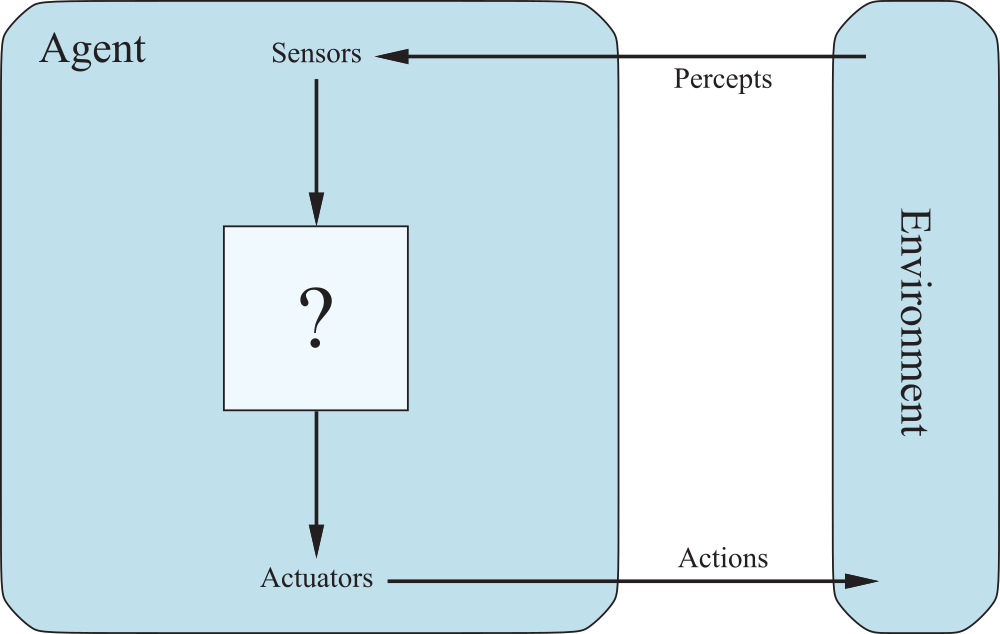
\includegraphics{Images/Chapter 1/agent-environment-schema.png}
    \caption{Schema of the interaction between an agent and the environment.}
    \source{Russel and Norvig, 2020}
    \label{fig:ch1-agentenvironmentschema}
\end{figure}
\begin{figure}[hbtp]
    \centering
    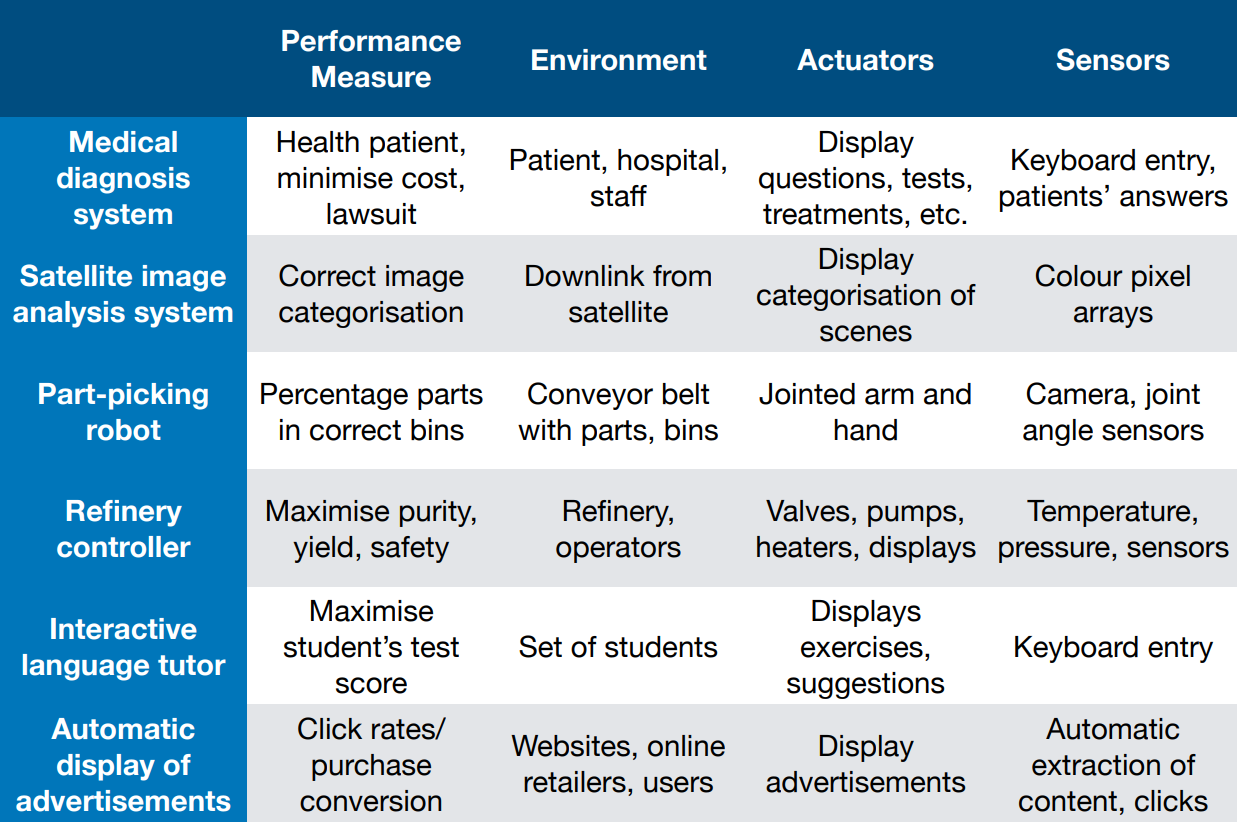
\includegraphics[width=\textwidth]{Images/Chapter 1/agents-type.png}
    \caption{Examples of agents and their characteristics.}
    \source{Prof. Mirco Musolesi}
    \label{fig:ch1-agentexamples}
\end{figure}

\section{Characteristics of the environments}
The environment in which our agent is situated may be of different types:

\begin{itemize}
    \item \textbf{Fully observable vs partially observable}: we may or may not be able to see the entire environment (e.g., there may be occlusions limiting our sight).
    \item \textbf{Deterministic vs stochastic}: the environment may be predictable (e.g., governed by the laws of Newtonian physics) or not (e.g., the environment may be subject to changes performed by another agent).
    \item \textbf{Episodic vs sequential}: the environment may be divided in “episodes” that have a beginning and an end (e.g., the levels of a game) or open-ended (e.g., a self-driving car that keeps on driving).
    \item \textbf{Static vs dynamic}: the environment may or may not change over time (an action that we take now could have a different result compared to when we took it in the past, e.g., certain agents with whom we collaborated in the past, may not do so anymore; driving in dry conditions is different compared to driving in the rain or in the snow; etc.).
    \item \textbf{Discrete vs continuous}: the environment may be represented by means of discrete or continuous values (e.g., a switch can be ON or OFF; the wind speed might be 14.6 km/h from N/E; etc.).
    \item \textbf{Single-agent or multi-agent}: there may be multiple agents in the environment, and we might want them to collaborate.
\end{itemize}

\section{A categorization of intelligent agents}
There are essentially four basic kinds of agents:

\begin{itemize}
    \item \textbf{Simple reflex agents}.
    \item \textbf{Model-based reflex agents}.
    \item \textbf{Goal-based agents}.
    \item \textbf{Utility-based agents}.
\end{itemize}

The behavior of these agents can be hard-wired, or it can be acquired, improved, and optimized through learning.

\subsection{Simple reflex agents}
Simple reflex agents (figure \ref{fig:ch1-simplereflexagent}) select actions on the basis of the current perceptions, ignoring the perception history. They are the most basic form of agents and are based on condition-action rules (also called \textbf{stimulus-response} rules, productions, or if-then rules).

\begin{figure}[hbt]
    \centering
    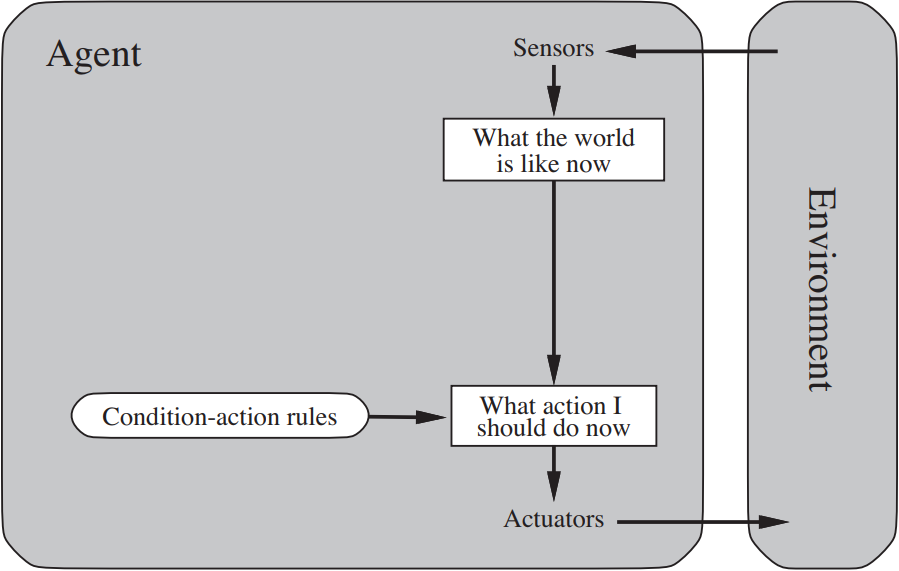
\includegraphics{Images/Chapter 1/simple-reflex-agents.png}
    \caption{Schema of a simple reflex agent.}
    \source{Russel and Norvig, 2020}
    \label{fig:ch1-simplereflexagent}
\end{figure}

\subsection{Model-based reflex agents}
Model-based agents (figure \ref{fig:ch1-modelbasedreflexagent}) keep an internal state and depend on two types of knowledge:

\begin{itemize}
    \item How the world evolves independently from the agent (e.g., the trajectory that a bullet/a stone follows when shot/thrown).
    \item How the actions of the agent affect the world (e.g., if I turn the wheel to the right, the car moves to the right).
\end{itemize}

The internal state is essentially used to keep track of what it is not possible to see/perceive at the current time. It depends on the perception history and, for this reason, it reflects at least some of the unobserved aspects of the current state.

\begin{figure}[hbtp]
    \centering
    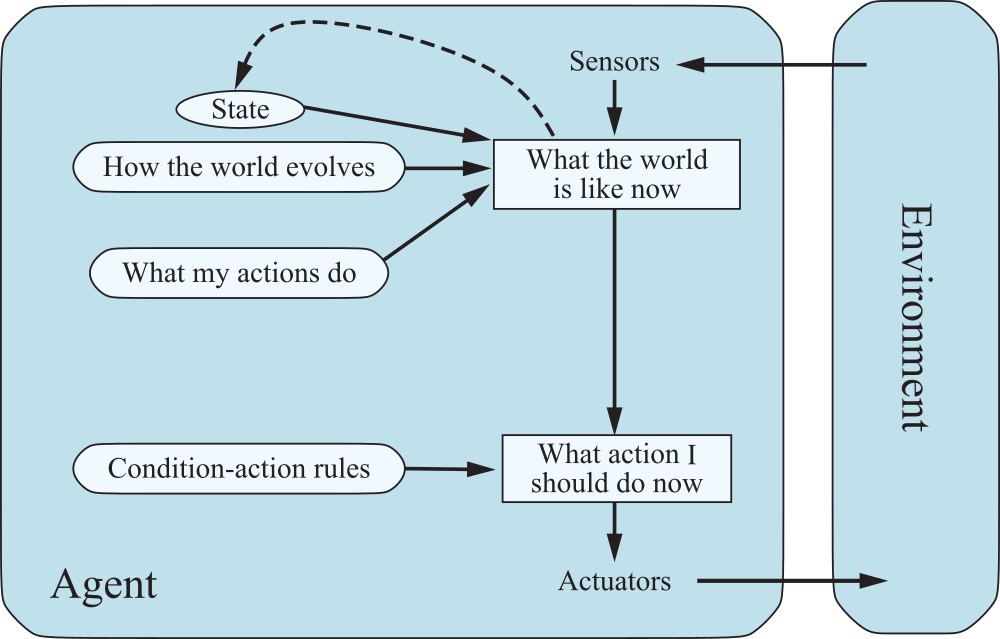
\includegraphics{Images/Chapter 1/model-based-reflex-agent.png}
    \caption{Schema of a model-based reflex agent.}
    \source{Russel and Norvig, 2020}
    \label{fig:ch1-modelbasedreflexagent}
\end{figure}

\subsection{(Model-based) Goal-based agents}
Goal-based agents (figure \ref{fig:ch1-goalbasedagent}) act in order to achieve their goals. If we can achieve the goal by carrying out a single action, goal-based action selection is straightforward; in the other cases, the agent needs to consider a long sequence of actions by means of search and planning.

\begin{figure}[hbtp]
    \centering
    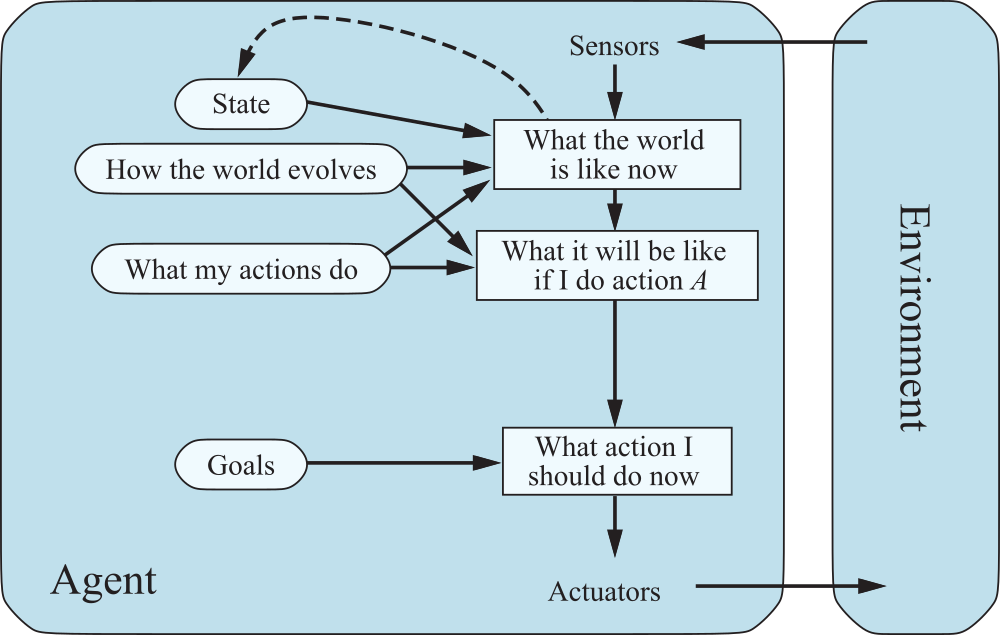
\includegraphics{Images/Chapter 1/goal-based-agent.png}
    \caption{Schema of a goal-based agent.}
    \source{Russel and Norvig, 2020}
    \label{fig:ch1-goalbasedagent}
\end{figure}

\subsection{(Model-based) Utility-based agents}
Goals are not sufficient to generate high-quality behavior in most environments, since there are usually states that are preferrable to others. In order to code this preference, we use utility functions that map a state (or a sequence of states) to a real number (e.g., we want to get to a destination by following the shortest or quickest path). (See figure \ref{fig:ch1-utilitybasedagent})

Note that how to model these preferences is one of the current unsolved and “hot” topics in the artificial intelligence field.

\begin{figure}[hbtp]
    \centering
    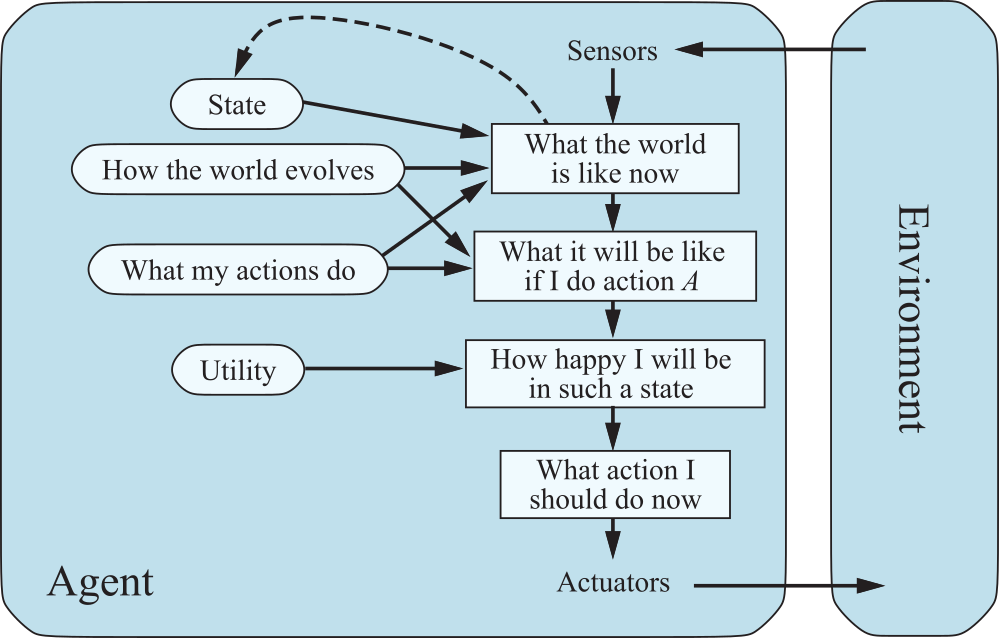
\includegraphics{Images/Chapter 1/utility-based-agent.png}
    \caption{Schema of a utility-based agent.}
    \source{Russel and Norvig, 2020}
    \label{fig:ch1-utilitybasedagent}
\end{figure}

To conclude this first introduction, let us quickly consider the topic of learning.

\section{Learning}
As we said before, the behavior of the agents can be pre-programmed (hard-wired, fixed) or it can be learned by means of a learning component. This component can be based on a model of the world and the gain towards a certain goal can be expressed through rewards. This behavior is at the basis of the type of learning that we will explore in detail in this course, called \textbf{reinforcement learning}. Following Herbert Simon’s definition of autonomous and adaptive systems, we will consider \textit{``machines that think, that learn and that create''}.
\chapter{Introduction to Reinforcement Learning}
The Merriam-Webster dictionary defines learning as the \textit{``modification of a behavioral tendency by experience''}\footnote{\url{https://www.merriam-webster.com/dictionary/learning}}. Interacting with the external world to learn, in fact, is an idea that is at the basis of nearly all theories of learning and intelligence. In the artificial intelligence world, this approach is leveraged with success in reinforcement learning.

\textbf{Reinforcement learning is learning what to do and how to map situations to actions, so as to maximize a numerical reward} (it is goal-directed learning from interaction). The learner is not told which actions to take, but instead it must discover which actions yield the most reward by trying them out. In the most interesting and challenging cases, actions may affect not only the immediate reward but also the next situation and, through that, all subsequent rewards. These two characteristics (trial-and-error search and delayed reward) are the two most important distinguishing features of reinforcement learning.

We will now introduce finite Markov decision processes, a mathematical framework that we are going to use.

\section{Finite Markov Decision Processes}
Markov Decision Processes (MDPs) are a mathematically idealized formulation of reinforcement learning for which precise theoretical statements can be made. They provide a mathematical framework for modeling decision making in situations where outcomes are partly random and partly under the control of a decision maker\footnote{See \url{https://en.wikipedia.org/wiki/Markov_decision_process}}.

At each time step $t$, the process is in some state $s$, and the decision maker may choose an action $a$ that is available in state $s$. The process responds at the next time step by randomly moving into a new state $s'$, and giving the decision maker a corresponding reward $R_a(s,s')$. The probability that the process moves into its new state $s'$ is influenced by the chosen action. Specifically, it is given by the state transition function $P_a(s,s')$. Thus, the next state $s'$ depends on the current state $s$ and the decision maker's action $a$. But \textbf{given $\boldsymbol{s}$ and $\boldsymbol{a}$, it is conditionally independent of all previous states and actions}; in other words, the state transitions of an MDP satisfy the Markov property \textit{(memoryless property of a stochastic process)}.

\begin{figure}[hbt]
    \centering
    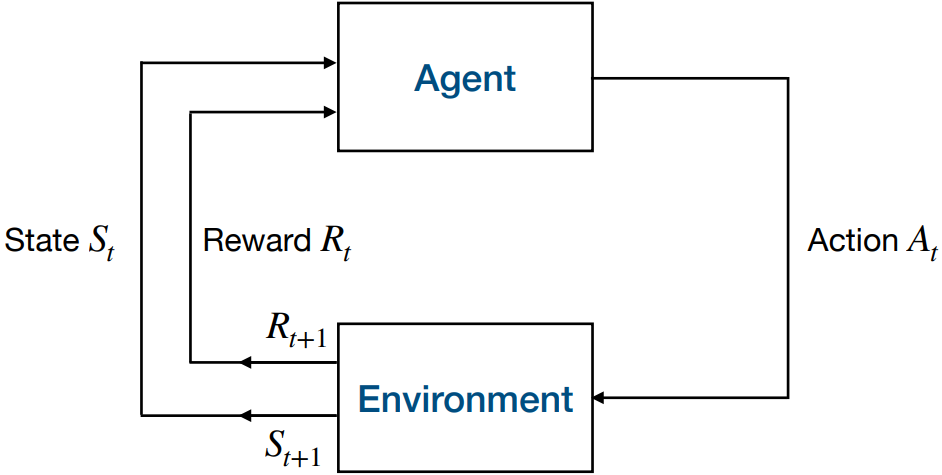
\includegraphics[width=\textwidth]{Images/Chapter 2/mdp.png}
    \caption{Schema of a Markov Decision Process.}
    \source{Prof. Mirco Musolesi}
    \label{fig:ch2-mdp}
\end{figure}

\section{Rewards and expected returns}
Informally, the agent’s goal is to maximize the \textbf{total amount} of rewards it receives (note how the agent should not maximize the immediate reward, but the cumulative reward). We can formalize this with the \textbf{``reward hypothesis''}: \textit{``That all of what we mean by goals and purposes can be well thought of as the maximization of the expected value of the cumulative sum of a received scalar signal (called reward)''}.

We will now try to conceptualize the idea of \textbf{cumulative rewards} more formally by means of the notion of \textbf{expected return} $\boldsymbol{G_t}$. To do so, we first need to distinguish between two cases:

\begin{itemize}
    \item \textbf{Episodic tasks}, in which we can identify a final step of the sequence of rewards (i.e., in which the interaction between the agent and the environment can be broken into sub-sequences called \textbf{episodes}, such as playing a game, repeated tasks, etc.). Each episode ends in a terminal state after $T$ steps, followed by a reset to a standard starting state or to a sample of a distribution of starting states (the next episode will be completely independent from the previous one).
    \item \textbf{Continuous tasks}, in which the agent-environment interaction does not break naturally into identifiable episodes, but goes on continually without limit (e.g., an ongoing monitoring of a process).
\end{itemize}

The expected return $G_t$ associated to the selection of an action $A_t$, assuming that the agent receives over time a sequence of rewards $R_{t+1}, R_{t+2}, R_{t+3}, ...$ is defined as:

\begin{itemize}
    \item The \textbf{sum of future rewards} in the case of \textbf{episodic tasks}:
    \begin{equation}
        G_t \doteq R_{t+1} + R_{t+2} + R_{t+3} + ... + R_T
        \label{eq:ch2-expectedreturn-episodic}
    \end{equation}
    \item The \textbf{discounted sum of future rewards} in the case of \textbf{continuing tasks}:
    \begin{equation}
        G_t \doteq R_{t+1} + \gamma R_{t+2} + \gamma^2 R_{t+3} + ... = \sum_{k=0}^{\infty} \gamma^k R_{t+k+1}
        \label{eq:ch2-expectedreturn-continuous}
    \end{equation}
\end{itemize}

Where $\gamma$ is the \textbf{discount rate}, with $0 \le \gamma \le 1$. The discount rate is used to give more importance to the rewards that are closer to us in time; this is particularly useful in dynamic environments. The definition of expected return that we used for episodic tasks would in fact be problematic for continuing tasks: the expected return would be equal to $\infty$ (in the limit of an infinite number of time steps) in some cases, such as when the reward is equal to $1$ at each time step. The discount rate then determines the ``present value of future rewards'' (how much future rewards mean to us at the current time): a reward received $k$ time steps in the future is worth $\gamma^{k-1}$ of what it would be worth if it were received immediately.

Returns at successive time steps are related to each other as follows:

\begin{equation*}
    \begin{split}
        G_t & \doteq R_{t+1} + \gamma R_{t+2} + \gamma^2 R_{t+3} + \gamma^3 R_{t+4} + ... \\
        & = R_{t+1} + \gamma \left( R_{t+2} + \gamma R_{t+3} + \gamma^2 R_{t+4} + ... \right) \\
        & = R_{t+1} + \gamma G_{t+1} \\
    \end{split}
\end{equation*}

\section{Policies and value functions}
Almost all reinforcement learning algorithms involve estimating value functions, i.e., functions of states (or of state-action pairs) that estimate how good it is for the agent to be in a given state (or how good it is to perform a given action in a given state). The notion of ``how good'' here is defined in terms of future rewards that can be expected, or, to be precise, in terms of expected return.

A \textbf{policy} is used to model how the agent will behave based on the previous experience and the rewards an agent received in the past (and, consequently, the expected returns). Formally, a policy is a mapping from states to probabilities of taking each possible action (the probability of taking a certain action in a certain state). If the agent is following the policy $\pi$ at time $t$, then $\pi (a \vert s)$ is the probability that $A_t=a$ if $S_t=s$.

\textbf{The value function of a state $\boldsymbol{s}$ under a policy $\boldsymbol{\pi}$}, denoted $v_\pi (s)$, is the expected return when starting in $s$ and following $\pi$ thereafter (the expected return I can have in the future state, considering all the actions I might take from there). For Markov Decision Processes, we can define \textbf{the state-value function} $\boldsymbol{v_\pi}$ for the policy $\pi$ formally as:

\begin{equation}
    v_\pi(s) \doteq \mathbb{E}_\pi \left[ G_t  \ \vert \  S_t = s \right] = \mathbb{E}_\pi \left[ \sum_{k=0}^{\infty}  \gamma^k R_{t+k+1} \  \middle\vert \  S_t = s, A_t = a \right] \quad \forall s \in \mathcal{S}
    \label{eq:ch2-statevaluefunction}
\end{equation}

Where $\mathbb{E}_\pi [\cdot]$ denotes the expected value of a random variable given that the agent follows $\pi$ and $t$ is any time step. Note that the value of the terminal state, if any, is always $0$. The formula above denotes a weighted average of the expected value (it is averaged because the values depend on the probability of a certain action being taken, which is a fraction).

Similar to what we just did, we can define \textbf{the action-value function}, i.e., the value of taking an action $a$ in the state $s$ under a policy $\pi$, denoted $\boldsymbol{q_\pi (s,a)}$, as the expected return starting from $s$, taking the action $a$, and following the policy $\pi$ thereafter:

\begin{equation}
    q_\pi(s,a) \doteq \mathbb{E}_\pi \left[ G_t \  \vert \  S_t = s, A_t = a \right] = \mathbb{E}_\pi \left[ \sum_{k=0}^{\infty} \gamma^k R_{t+k+1} \  \middle\vert \ S_t = s, A_t = a \right]
    \label{eq:ch2-actionvaluefunction}
\end{equation}

\section{Choosing the rewards}
When we model a real system as a reinforcement learning problem, the most difficult task is selecting the right rewards. Typically, we use negative values for actions that do not help us in reaching our goal, and positive if they do (it is also possible using 0 as a value for actions that do not help us). An alternative is to set the values of the rewards to a negative number until we reach our goal (using 0 as the value when we reach it).

When choosing the rewards, it is very important that \textbf{we should not ``reward'' the intermediate steps or the single actions}. The agent, in fact, always learns to maximize its reward. If we want it to do something for us, we must provide rewards to it in such a way that in maximizing them the agent will also achieve our goals. It is thus critical that the rewards we set up truly indicate what we want accomplished. If we were to give importance to certain sub-goals, the agent might find a way to achieve them without achieving the real goal (e.g., taking the opponent's pieces while playing chess but losing the game). Note that the reward signal is our way of communicating to the agent \textit{what} we want achieved, not \textit{how} (a better place for imparting this kind of prior knowledge would be the initial policy or the initial value function).

Giving rewards to the agent could be a challenging task, as we will see from the two examples that follow. Let us first imagine that we want to create an agent that completes a maze in the least time possible: we could give a reward of -1 for every step it takes inside the maze and 0 for reaching the exit. This could work even if we assume that we only have one episode to base our rewards on. There are situations, though, in which we need additional information to quantify how good an action is for us, like in a game of chess, where we can only assign the rewards at the end of the game (e.g., assigning 1 to every step if we won, -1 if we lost). This is usually called \textbf{credit assignment problem} (i.e., the problem of assigning a reward to each step) and a discussion on it can be found in Marvin Minsky’s ``Steps Towards Artificial Intelligence'' paper \cite{4066245}.

We now need to think about how we can solve this problem and estimate the value functions $v_\pi$ and $q_\pi$. If the behavior of the Markov Decision Process is known (i.e., the transition probabilities between all the states are known), we could do so by considering all the possible moves, although this poses strict requirements in terms of prior knowledge and system complexity. A more general option is to estimate them through experience: if an agent follows policy $\pi$ and maintains an average, for each state encountered, of the actual returns that have followed that state, then the average will converge asymptotically to the state’s value, $v_\pi(s)$, as the number of times that that state is encountered approaches infinity (these methods are referred to as \textbf{Monte Carlo methods} because they involve averaging over many random samples of actual returns). This option is still problematic when it comes to very large number of states, though, as it would involve keeping separate averages for each state individually. In those cases, instead, we will maintain $v_\pi$ and $q_\pi$ as parametrized functions, with fewer parameters than the number of states, using approximators such as artificial neural networks.

\section{Optimal policies and optimal value functions}
Solving a reinforcement learning task is roughly equivalent to finding a policy that maximizes the reward in the long run. In finite Markov Decision Processes, there is always at least one policy $\pi$ that is better than (or equal to) all the other policies, meaning that its expected return is greater than (or equal to) that of a different policy $\pi'$ for all states. More formally:

\begin{equation*}
    \pi \ge \pi' \text{ if and only if } v_\pi(s) \ge v_{\pi'} (s) \quad \forall s \in \mathcal{S}
\end{equation*}

Although there may be more than one, we denote all the optimal policies with $\pi_*$. They share the same state-value function, called the \textbf{optimal state-value function}, denoted $v_*$ and defined as:

\begin{equation}
    v_*(s) \doteq \max_\pi v_\pi(s) \quad \forall s \in \mathcal{S}
    \label{eq:ch2-optimalstatevaluefunction}
\end{equation}

This means that, given a state and the value function, the optimal policy is the one that gives us the maximum reward. The same goes for the \textbf{optimal action-value function}, denoted $q_*$ and defined as:

\begin{equation}
    q_*(s,a) \doteq \max_\pi q_\pi(s,a) \quad \forall s \in \mathcal{S}, a \in \mathcal{A}(s)
    \label{eq:ch2-optimalactionvaluefunction}
\end{equation}

For the state-action pair $(s,a)$, this function gives the expected return for taking the action $a$ in the state $s$ and thereafter following an optimal policy. Thus, we can write $q_*$ in terms of $v_*$ as follows:

\begin{equation*}
    q_*(s,a) = \mathbb{E}_{\pi} \left[ R_{t+1} + \gamma v_* S_{t+1} \  \middle\vert \ S_t = s, A_t = a \right]
\end{equation*}

\section{Optimality and approximation}
\subsection{Bellman equation}
What we are doing is closely related to the issues of automatic control: we both want to have knowledge and control over the evolution of a system.

For any policy $\pi$ and any state $s$, the following consistency condition holds between the value of $s$ and the value of its possible successor states:

\begin{equation}
    \begin{split}
        v_\pi(s) & \doteq \mathbb{E}_\pi \left[ G_t \ \vert \ S_t = s \right] \\
        & = \mathbb{E}_\pi \left[ R_{t+1} + \gamma G_{t+1} \ \vert \ S_t = s \right] \\
        & = \sum_{a} \pi(a \vert s) \sum_{s'} \sum_{r} p(s',r \ \vert \ s,a) \Big[ r + \gamma \mathbb{E}_\pi \left[ G_{t+1} \ \vert \ S_{t+1} = s' \right] \Big] \\
        & = \sum_{a} \pi (a \vert s) \sum_{s', r} p(s', r \ \vert \ s,a) \Big[ r + \gamma v_\pi(s') \Big], \quad \forall s \in \mathcal{S}
    \end{split}
    \label{eq:ch2-bellmanequation}
\end{equation}

What we have in the end is known as the \textbf{Bellman equation} for $v_\pi$ and it states that the value of the start state must equal the (discounted) value of the expected next state, plus the reward expected along the way.

\subsection{Bellman optimality equation}
We can re-write the Bellman equation under the optimal policy, obtaining what is known as the \textbf{Bellman optimality equation}:

\begin{equation}
    \begin{split}
        q_*(s,a) & = \mathbb{E}_{\pi} \left[ R_{t+1} + \gamma \max_{a'} q_* (S_{t+1}, a') \ \middle\vert \ S_t = s, A_t = a \right] \\
        & = \sum_{s', r} p(s',r \ \vert \ s,a) \left[ r + \gamma \max_{a'} q_*(s',a') \right]
    \end{split}
    \label{eq:ch2-bellmanoptimalityequation}
\end{equation}

Intuitively, the Bellman optimality equation must equal the expected return for the best action from that state. 

The Bellman optimality equation is actually a system of equations, one for each state, so if there are $n$ states, then there are $n$ equations in $n$ unknowns. If the dynamics $p$ of the environments are known, then in principle one can solve this system of equation for $v_*$. Once we have $v_*$ (or $q_*$), the actions that select the highest value for them in each state will then be the optimal actions. Another way of saying this is that any policy that is \textbf{greedy} with respect to the optimal evaluation function is an optimal policy. As a reminder, the term \textit{greedy} is used in computer science to describe any search or decision procedure that selects alternatives based only on local or immediate considerations, without considering the possibility that such a selection may prevent future access to even better alternatives. This is not an issue in the case of Markov Decision Processes, though, as they depend only on the current state: \textbf{a greedy policy is then optimal both in the short and in the long-term}.

As we were hinting at earlier, it may not always be possible to solve the Bellman optimality equations, both due to the huge number of states (and equations) involved in non-trivial problems and because the state may not be fully observable, or we may not be able to know its dynamics.
\chapter{Multi-Armed Bandits}
In this chapter we want to study the evaluative and explorative aspects of reinforcement learning in a simplified setting that does not involve learning to act in more than one situation.

\section{The k-armed bandit problem}
To do so, we introduce the \textbf{$\boldsymbol{k}$-armed bandit problem} (a slot machine with $k$ levers), where we must choose between $k$ different options (the $k$ arms of the bandit), and after each choice we receive a reward taken from a \textbf{stationary} probability distribution depending on the action we selected (the state is not taken into account). Our objective is to maximize the expected total reward over a certain number of time steps.

As a note, there is a different version of the $k$-armed bandit problem, known as \textbf{contextual bandits}, in which we do consider the state but assume that it does not depend on previous actions. This problem is at the basis of ad-serving platforms, and we will talk more about it at the end of this chapter.

Let us now see things from a more formal point of view: in our $k$-armed bandit problem, each of the $k$ actions has an expected (or mean) reward given that that action is selected; let us call this the \textit{value} of that action. We denote the action selected on time step $t$ as $A_t$, and the corresponding reward as $R_t$. Our goal is then to maximize the following:

\begin{gather*}
    \mathbb{E} \left[ G_t \  \middle\vert \  S_t = s, A_t = a \right] \doteq \mathbb{E} \left[ R_{t+1} + \gamma R_{t+2} + \gamma^2 R_{t+3} + ... \  \middle\vert \  S_t = s, A_t = a \right] \\
    = \mathbb{E} \left[ \sum_{k=0}^{\infty} \gamma^k R_{t+k+1} \  \middle\vert \  S_t = s, A_t = a \right]
\end{gather*}

Since in multi-armed bandits we do not consider the state, we can think of it as a constant $\bar{s}$ and substitute it in the formula above, obtaining:

\begin{gather*}
    \mathbb{E} \left[ G_t \  \middle\vert \  S_t = \bar{s}, A_t = a \right] \doteq \mathbb{E} \left[ R_{t+1} + \gamma R_{t+2} + \gamma^2 R_{t+3} + ... \  \middle\vert \  S_t = \bar{s}, A_t = a \right] \\
    = \mathbb{E} \left[ \sum_{k=0}^{\infty} \gamma^k R_{t+k+1} \  \middle\vert \  S_t = \bar{s}, A_t = a \right]
\end{gather*}

The value of an arbitrary action $a$ denoted as $q_*(a)$ is the expected reward given that $a$ is selected. More formally:

\begin{equation*}
    q_*(a) \doteq \mathbb{E} \left[ R_t \  \middle\vert \  A_t = a \right]
\end{equation*}

(Note how the expected reward does not include the state, as it is always the same). If we disregard the trivial case in which we already know the value of each action, we need to play to be able to estimate the value of the various actions: we denote the estimated value of action $a$ at time step $t$ as $Q_t(a)$ and we want it to be as close as possible to $q_*(a)$.

If we maintain the estimates of each action value, then at any time step there will be at least one action whose value is greater than --or equal to-- all the other ones (we refer to this action as the \textbf{greedy action}). When we select one of these actions, we are \textbf{exploiting our current knowledge} of the value of the actions. If instead we choose one of the nongreedy actions, we are \textbf{exploring}, as this enables us to improve our estimate of the nongreedy action’s value. Exploitation maximizes the expected reward on the step, but by exploring, we may obtain a greater total reward in the long run (this is particularly true if our estimates have high uncertainty). In any specific case, whether it is better to explore or exploit depends in a complex way on the precise values of the estimates, uncertainties, and the number of remaining steps.

\section{Evaluating action-value methods}
Now that we have understood the need for \textbf{action-value methods}, meaning methods that estimate the values of the available actions and use them to choose actions to take, we will look at some instances of these methods.

In the case of the $k$-armed bandits problem, the value of an action is the mean reward when that action is selected, since we only have one state. A possible way to estimate this is by averaging the rewards we actually received:

\begin{gather}
    Q_t(a) \doteq \frac{\text{sum of rewards when an action } a \text{ is taken prior to time } t}{\text{number of times an action } a \text{ is taken prior to time } t}\nonumber\\
    = \frac{\sum_{i=1}^{t-1} R_i \cdot \mathbbm{1}_{A_i = a}}{\sum_{i=1}^{t-1} \mathbbm{1}_{A_i = a}}
    \label{eq:ch3-sampleaveragemethod}
\end{gather}

Where $\mathbbm{1}_{\text{predicate}}$ denotes the random variable that is 1 if predicate is true and 0 if it is not. If the denominator is zero, then we instead define $Q_t(a)$  as some default value, such as 0. As the denominator goes to infinity, by the law of large numbers, $Q_t(a)$ converges to $q_*(a)$. We call this the \textbf{sample-average method} for estimating action values because each estimate is an average of the sample of relevant rewards.

When it comes to selecting actions, the simplest action selection rule is to select one of the actions with the highest estimated value, that is, one of the greedy actions. If there is more than one greedy action, then a selection is made among them in some arbitrary way, perhaps randomly. We can formalize this \textbf{greedy action selection method} as:

\begin{equation}
    A_t \doteq \argmax_a  Q_t(a)
    \label{eq:ch3-greedyactionselectionmethod}
\end{equation}

Where $\argmax_a$ denotes the action $a$ for which the expression that follows is maximized (with ties broken arbitrarily). The greedy action selection always exploits the current knowledge to maximize the immediate reward, disregarding exploration. To include it, we can add a small probability $\varepsilon$ where the next action is selected randomly from all the actions with equal probability. This is called the \textbf{$\boldsymbol{\varepsilon}$-greedy selection rule} and it has the advantage that in the limit, as the number of steps increases, every action will be sampled an infinite number of times, ensuring that all the $Q_t(a)$ converge to their respective $q_*(a)$ (these, however, are just asymptotic guarantees and say little about the practical effectiveness of these methods).

\section{Incremental implementation}
\label{section:incrementalimplementation}
We now move to the question of how the methods that we have seen before can be computed in a computationally efficient manner, with constant memory usage and computation time.

To simplify the notation, we will concentrate on a single action $a$. Let $R_i(a)$ denote the reward received after the $i$-th selection of the action $a$, and let $Q_n$ denote the estimate of its action value after it has been selected $n-1$ times. We can now write:

\begin{equation*}
    Q_n(a) \doteq \frac{R_1(a) + R_2(a) + ... + R_{n-1}(a)}{n-1}
\end{equation*}

A trivial implementation of this would be to maintain a record of all the rewards and then perform this computation whenever the estimate value is needed. However, both memory and computation requirements would grow over time as more and more rewards are received. This can be avoided by considering the following steps:

\begin{equation*}
    \begin{split}
        Q_{n+1} & = \frac{1}{n} \sum_{i=1}^{n} R_i\\
        & = \frac{1}{n} \Big( R_n + \sum_{i=1}^{n-1} R_i \Big) \\
        & = \frac{1}{n} \Big( R_n + (n-1) \frac{1}{n-1} \sum_{i=1}^{n-1} R_i \Big) \\
        & = \frac{1}{n} \Big( R_n + (n-1) Q_n \Big) \\
        & = \frac{1}{n} \Big( R_n + n Q_n - Q_n \Big) \\
        & = Q_n + \frac{1}{n} \Big[R_n - Q_n \Big]
    \end{split}
\end{equation*}

This type of update rule is quite common in reinforcement learning and follows this general formula:

\begin{equation}
    \text{NewEstimate} \leftarrow \text{OldEstimate} + \text{StepSize}(\text{Target} - \text{OldEstimate})
    \label{eq:ch3-generalrlupdaterule}
\end{equation}

The expression $(\text{Target} - \text{OldEstimate})$ is usually defined as the \textbf{error} in the estimate. It is reduced by taking a step towards the $\text{Target}$, which is presumed to indicate a desirable direction in which to move (though it may be noisy).

\section{Tracking a nonstationary problem}
The averaging method we just discussed is appropriate for stationary bandit problems, where the distribution of the rewards does not change over time. Many problems, however, fall in the nonstationary category and in those cases, it makes sense to give more weight to recent rewards, rather than long-gone ones. One of the most popular ways of dealing with these problems is using a \textbf{constant step-size parameter} $\boldsymbol{\alpha}$ in the range $]0,1]$, obtaining a formula such as the following:

\begin{equation}
    Q_{n+1} \doteq Q_n + \alpha \left[R_n - Q_n \right]
    \label{eq:ch3-nonstationaryincrementalupdaterule}
\end{equation}

\textbf{This results in $\boldsymbol{Q_{n+1}}$ being a weighted average of past rewards and the initial estimate $\boldsymbol{Q_1}$}, as we can see in the demonstration below:

\begin{equation}
    \begin{split}
        Q_{n+1} &= Q_n + \alpha \Big[ R_n - Q_n \Big] \\
        &= \alpha R_n + (1 - \alpha) Q_n \\
        &= \alpha R_n + (1 - \alpha) [\alpha R_{n-1} + (1 - \alpha) Q_{n-1}] \\
        &= \alpha R_n + (1 - \alpha) \alpha R_{n-1} + (1 - \alpha)^2 Q_{n-1} \\
        &= \alpha R_n + (1 - \alpha) \alpha R_{n-1} + (1 - \alpha)^2 \alpha R_{n-2} + ... + (1 - \alpha)^{n-1} \alpha R_1 + (1 - \alpha)^n Q_1 \\
        &= (1 - \alpha)^n Q_1 + \sum_{i=1}^{n} \alpha (1 - \alpha)^{n-i} R_i
    \end{split}
    \label{eq:ch3-exponentialrecencyweightedaverage}
\end{equation}

This is called a weighted average since the sum of the weights $(1 - \alpha)^n + \sum_{i=1}^{n} \alpha (1 - \alpha)^{n-i} = 1$, as we can see here:

\begin{equation*}
    \begin{split}
        & (1 - \alpha)^n + \sum_{i=1}^{n} \alpha (1 - \alpha)^{n-i} \\
        &= (1 - \alpha)^n + \alpha (1 - \alpha)^n \sum_{i=1}^{n} (1 - \alpha)^{-i} \\
        &= (1 - \alpha)^n + \alpha (1 - \alpha)^n \Big(-1 + \sum_{i=0}^{n} (1 - \alpha)^{-i} \Big) \\
        &= (1 - \alpha)^{n+1} + \alpha (1 - \alpha)^n \sum_{i=0}^{n} (1 - \alpha)^{-i} \\
        &= (1 - \alpha)^{n+1} + \alpha (1 - \alpha)^n \frac{\alpha + (1 - \alpha)^{-n} -1}{\alpha} \\
        &= (1 - \alpha)^{n+1} + (1 - \alpha)^n \Big( \alpha + (1 - \alpha)^{-n} -1 \Big) \\
        &= (1 - \alpha)^{n+1} + \alpha (1 - \alpha)^n + 1 - (1 - \alpha)^n \\
        &= (1 - \alpha)^{n+1} + (1 - \alpha)^n (\alpha - 1) + 1 \\
        &= (1 - \alpha)^{n+1} - (1 - \alpha)^{n+1} + 1 = 1
    \end{split}
\end{equation*}

The quantity $1 - \alpha$ is less than $1$, and thus the weight given to $R_i$ decreases as the number of rewards increases. In fact, the weight decreases exponentially according to the exponent on $1 - \alpha$; accordingly, this is sometimes called an \textbf{exponential recency-weighted average}.

\section{Optimistic initial values}
All the methods that we have discussed until now depend to some extent on the initial action-value estimates (they are \textbf{biased} by their initial estimates). For the sample-average methods, the bias disappears once all actions have been selected at least once, while for methods with a constant $\alpha$ the bias is permanent (although decreasing over time as given by the equation \ref{eq:ch3-exponentialrecencyweightedaverage}). In practice, this kind of bias is usually not a problem and can sometimes be helpful, especially to supply some prior knowledge or to encourage exploration. The downside is that the initial estimates become, in effect, a set of parameters that must be picked by the user.

Choosing a wildly optimistic initial value encourages action-value methods to explore: whichever actions are initially selected, the reward is less than the starting estimates; the learner will then switch to other actions, being ``disappointed'' with the rewards it is receiving. The result is that all actions are tried several times before the value estimates converge, making the system do a fair amount of exploration even with a fully greedy action selection strategy. Initially, the optimistic method performs worse because it explores more, but eventually it performs better as its exploration decreases with time. We call this technique for encouraging exploration \textbf{optimistic initial values}. It is a simple trick that can be quite effective on stationary problems, while it is not well suited to nonstationary problems, as its drive for exploration is inherently temporary (any method that focuses on the initial conditions is unlikely to help with the general nonstationary case).

\section{Upper-Confidence-Bound Action Selection}
Exploration is needed because there is always uncertainty about the accuracy of the action-value estimates. $\varepsilon$-greedy action selection forces non-greedy (exploratory) actions to be tried, but indiscriminately, with no preference for those that are nearly greedy or particularly uncertain. It would be better to select among the non-greedy actions according to their potential for actually being optimal, taking into account both how close their estimates are to being maximal and the uncertainties in those estimates. One effective way of doing this is to select actions according to the following formula:

\begin{equation}
    A_t \doteq \argmax_a \Bigg[ Q_t (a) + c + \sqrt{\frac{\ln{t}}{N_t (a)}} \Bigg]
    \label{eq:ch3-upperconfidenceboundactionselection}
\end{equation}

Where $t$ is the time at which action $A_t$ is taken, $N_t (a)$ denotes the number of times that action a has been selected prior to time $t$ and the number $c > 0$ controls the degree of exploration. The idea of this \textbf{upper confidence bound (UCB)} action selection is that the square-root term is a measure of the uncertainty or variance of the estimate of the actual value of action $a$. The quantity being maxed over is thus a sort of upper bound on the possible true value of action $a$, with $c$ determining the confidence level. Each time $a$ is selected, the uncertainty is presumably reduced: $N_t (a)$ increments, and, as it appears in the denominator, the uncertainty term decreases. On the other hand, each time an action other than $a$ is selected, $t$ increases but $N_t (a)$ does not; because $t$ appears in the numerator, the uncertainty estimate increases. The use of the natural logarithm means that the increases get smaller over time, but are unbounded; all actions will eventually be selected, but actions with lower value estimates, or that have already been selected frequently, will be selected with decreasing frequency over time.

\section{Contextual bandits}
Multi-armed bandits are used when the selection of the action does not depend on the state, but for many application (e.g., ads on a webpage), the state is very important. When the action selection depends on the state, but not on its previous history, we speak of \textbf{contextual bandits}. They are examples of \textbf{associative search tasks}, as they involve both trial-and-error learning to \textbf{search} for the best actions, and \textbf{association} of these actions with the situation in which they are best (e.g., if we are on a website about sportscars, we will be served ads about cars and not about flowers). Contextual bandits are still not a ``full'' reinforcement learning problem, as actions do not affect the future state, but only the immediate reward.
\chapter{Monte Carlo Methods}
Monte Carlo methods are ways of solving the reinforcement learning problem based on averaging sample returns. To ensure that well-defined returns are available, we will focus on episodic tasks. That is, we assume experience is divided into episodes, and that all episodes eventually terminate no matter what actions are selected. Only on the completion of an episode are value estimates and policies changed. Monte Carlo methods can thus be incremental in an episode-by-episode sense, but not in a step-by-step (online) sense.

Monte Carlo methods sample and average \textbf{returns} for each state-action pair much like the bandit methods we explored earlier sample and average \textbf{rewards} for each action. The main difference is that now there are multiple states, each acting like a different (but interrelated) bandit problem. That is, \textbf{the return after taking an action in one state depends on the actions taken in later states in the same episode} (it is the \textbf{average expected cumulative reward}). 

From this point on, we will assume that we do not have full knowledge of the underlying Markov Decision Process. We are then entering the \textbf{full reinforcement learning problem}, in which the underlying dynamics and characteristics of the system are unknown (e.g., robot exploration) or because the system is too complex (e.g., games). In these types of problems, we will have to \textbf{learn the value functions from sample returns}.

We will consider three problems:
\begin{enumerate}
    \item The \textbf{prediction problem}, where we want to estimate $v_\pi$ and $q_\pi$ for a fixed policy $\pi$. We are given a fixed policy (that is, we know how we play) and we try to estimate the expected cumulative reward.
    \item The \textbf{policy improvement problem}, where we still try to estimate $v_\pi$ and $q_\pi$, but this time we also try to improve the policy $\pi$. We try to estimate the value of each state and we use this information to play better.
    \item The \textbf{control problem}, where we try to estimate an optimal policy $\pi_*$ (e.g., we try to find the best way to play a game; the best way to build a datacenter to minimize energy consumption; …).
\end{enumerate}

\section{Monte Carlo Prediction}
We begin by considering Monte Carlo methods for learning the state-value function for a given policy. Before doing so, we must have clear in our minds that \textbf{the value of a state is the expected return (expected cumulative future discounted reward) starting from that state}. An obvious way to estimate it from experience, then, is simply to average the returns observed after visits to that state. As more returns are observed, the average should converge to the expected value. This idea underlies all Monte Carlo methods.

More formally: we want to estimate $v_\pi (s)$, the value of a state $s$ under policy $\pi$, given a set of episodes obtained by following $\pi$ and passing through $s$. Each occurrence of state $s$ in an episode is called a \textbf{visit} to $s$. The same state may be visited multiple times in a certain episode: let us call the first time this happens the \textbf{first visit to} $\boldsymbol{s}$. The \textbf{first-visit Monte Carlo method} estimates $v_\pi (s)$ as the average of the returns following the \textit{``first visits''} to $s$, whereas the \textbf{every-visit Monte Carlo method} averages the returns following \textit{all visits} to $s$.

\subsection{First-visit Monte Carlo Prediction}
The algorithm for the \textit{first-visit Monte Carlo Prediction} is shown here:

\begin{algorithm}[H]
\SetAlgoLined
\KwIn{a policy $\pi$ to be evaluated}
\Initialize{
    \\
    \Indp % add indent
    $V(s) \in \mathbb{R}$, arbitrarily, $\forall s \in \mathcal{S}$ \\
    $Returns(s) \leftarrow $ an empty list, $\forall s \in \mathcal{S}$ \\
    \Indm % remove indent
}

 \Loop{forever (for each episode)}{
    Generate an episode following $\pi$: $S_0, A_0, R_1, ..., S_{T-1}, A_{T-1}, R_T$\\
    $G \leftarrow 0$\;
    \Loop{for each step of the episode, $t = T-1, T-2, ..., 0$}{
        $G \leftarrow \gamma G + R_{t+1}$\;
        \Unless{$S_t$ appears in $S_0, S_1, ..., S_{t-1}$}{
            Append $G$ to $Returns(s)$\;
            $V(S_t) \leftarrow average(Returns(S_t))$\;
        }
    }
    
 }
 \caption{First-visit Monte Carlo Prediction}
\end{algorithm}

This means generating an episode where we play following policy $\pi$ (the set of probabilities associated to each action) and analyzing the ``trajectory'' that we followed during the game in a backwards manner. During this phase we will calculate the values for all the states that we traversed and the average cumulative reward we can expect from them.

\subsection{Every-visit (multi-visit) Monte Carlo Prediction}
If we remove from the \textit{first-visit Monte Carlo Prediction} algorithm the check on whether a state $S_t$ has already occurred, we obtain the \textbf{every-visit Monte Carlo Prediction}, which also converges to $v_\pi (s)$ as the number of visits to a certain state $s$ goes to infinity.

\section{Monte Carlo Estimation of Action Values}
The estimation of a state value makes sense when we have a model of the system: with it, in fact, state values alone are sufficient to determine a policy; one simply looks ahead one step and chooses whichever action leads to the best combination of reward and next state. Without a model, however, it is necessary to estimate the value of each action in order for the value to be useful in suggesting a policy. 

The \textbf{policy evaluation problem} for action values is to estimate $q_\pi (s,a)$, the expected return when starting in state $s$, taking action $a$ and then following policy $\pi$. The methods for the Monte Carlo estimation of action values are essentially the same as those presented for state values, except that now we talk about \textbf{visits to the state-action pair} rather than to a state. A state-action pair $s,a$ is said to be visited in an episode if ever the state $s$ is visited and the action $a$ is taken in it. The first-visit Monte Carlo method averages the returns following the first time in each episode that the state was visited and the action was selected.

The only complication is that many state-action pairs may never be visited: if $\pi$ is a deterministic policy (to a certain state corresponds one and only one action), in fact, we would observe returns only for one of the actions of each state. With no returns to average, the Monte Carlo estimates of the other actions would subsequently not improve with experience. In order to compare alternatives, we then need to estimate the value of all the actions from each state, not only the one that is favored by our policy. This is the general problem of \textbf{maintaining exploration}.

For policy evaluation to work for action values, we must assure \textbf{continual exploration}. One way to do this is by specifying that the episodes start in a state-action pair, and that every pair has a nonzero probability of being selected as the start. This guarantees that all state-action pairs will be visited an infinite number of times in the limit of an infinite number of episodes; we call this the assumption of \textbf{exploring starts}. This assumption is sometimes useful, but it cannot be relied upon in general (we may need to enumerate all the states, or they may not be valid): the most common alternative approach is to assure that all state-action pairs are encountered. This means \textbf{not following the current policy} (for example by using a stochastic policy). In other words, the exploration is not performed \textbf{on-policy}, but \textbf{off-policy} (various methods are possible, like \textit{Off-policy Predictions via Importance Sampling}).

\section{Monte Carlo Policy Improvement and Monte Carlo Control}
So far, we have assumed that the policy $\pi$ was fixed, like in the case of a statically defined set of probabilities for each action (the \textit{prediction problem}). However, by using methods typically known as \textbf{Monte Carlo Control}, we can improve the policy and reach the optimal one. In this section we will focus on \textbf{on-policy methods}, meaning \textbf{methods that attempt to evaluate or improve the policy that is used to make decisions}.

The overall idea is to proceed according to the \textbf{Generalized Policy Iteration (GPI)}, in which we maintain both an approximate policy and an approximate value function. The value function is repeatedly altered to more closely approximate the value function for the current policy, and the policy is repeatedly improved with respect to the current value function. As we can imagine, these two changes work against each other to some extent, as each creates a ``moving target'' for the other, but together they cause both policy and value function to approach optimality.

With this method, we perform alternating complete steps of policy evaluation and policy improvement, beginning with an arbitrary policy $\pi_0$ and ending with the optimal policy and action-value function as such:

\begin{equation}
    \pi_0 \overset{E}{\rightarrow} q_{\pi_0} \overset{I}{\rightarrow} \pi_1 \overset{E}{\rightarrow} q_{\pi_1} \overset{I}{\rightarrow} \pi_2 \overset{E}{\rightarrow} ... \overset{I}{\rightarrow} \pi_* \overset{E}{\rightarrow} q_*
    \label{eq:ch3-generalizedpolicyiteration}
\end{equation}

Where $\overset{E}{\rightarrow}$ denotes a complete policy evaluation and $\overset{I}{\rightarrow}$ denotes a complete policy improvement. \textit{Policy evaluation} is performed as we mentioned in previous sections: many episodes are experienced, with the approximate action-value function approaching the true function asymptotically. \textit{Policy improvement} is done by making the policy greedy with respect to the current value function. Note how, since we have an action-value function, we do not need any model to construct the greedy policy: for any action-value function $q$, the corresponding greedy policy is the one that for each $s \in \mathcal{S}$, deterministically chooses an action with maximal action-value as such:

\begin{equation*}
    \pi(s) \doteq \argmax_a q(s,a)
\end{equation*}

Policy improvement can then be done by constructing each $\pi_{k+1}$ as the greedy policy with respect to $q_{\pi_k}$. The \textbf{policy improvement theorem} assures us that each $\pi_{k+1}$ is uniformly better than $\pi_k$ or just as good (in which case they are both optimal policies). This confirms that \textbf{the overall process converges to the optimal policy and optimal value function}.

\subsection{Monte Carlo Control algorithm with Exploring Starts}
Since we need to guarantee that all actions are selected ``infinitely often'', in some cases we can do so by means of \textbf{exploring starts}. A possible implementation of the \textbf{Monte Carlo Control algorithm with Exploring Starts} is shown in the box below:

\begin{algorithm}[H]
\SetAlgoLined
\Initialize{
    \\
    \Indp % add indent
    $\pi(s) \in \mathcal{A}(s)$ (arbitrarily), $\forall s \in \mathcal{S}$ \\
    $Q(s,a) \in \mathbb{R}$ (arbitrarily), $\forall s \in \mathcal{S}, a \in \mathcal{A}(s)$ \\
    $Returns(s,a) \leftarrow $ an empty list, $\forall s \in \mathcal{S}, a \in \mathcal{A}(s)$ \\
    \Indm % remove indent
}

 \Loop{forever (for each episode)}{
    Choose a starting state and action $S_0 \in \mathcal{S}, A_0 \in \mathcal{A}(S_0)$ randomly, such that all pairs have probability $> 0$\;
    Generate an episode starting with $S_0,A_0$ and following $\pi$: $S_0, A_0, R_1, ..., S_{T-1}, A_{T-1}, R_T$\;
    $G \leftarrow 0$\;
    \Loop{for each step of the episode, $t = T-1, T-2, ..., 0$}{
        $G \leftarrow \gamma G + R_{t+1}$\;
        \Unless{the pair $S_t, A_t$ appears in $S_0, A_0, S_1, A_1, ..., S_{t-1}, A_{t-1}$}{
            Append $G$ to $Returns(S_t, A_t)$\;
            $Q(S_t,A_t) \leftarrow average(Returns(S_t,A_t))$\;
            $\pi(S_t) \leftarrow \argmax_a Q(S_t,a)$\;
        }
    }
    
 }
 \caption{Monte Carlo Control algorithm with Exploring Starts}
\end{algorithm}

With this algorithm, all the returns for each state-action pair are accumulated and averaged, irrespective of what policy was in force when they were observed. It is easy to see that it cannot converge to any suboptimal policy: if it did, then the value function would eventually converge to the value function for that policy, and that in turn would cause the policy to change. \textbf{Stability is achieved only when both the policy and the value function are optimal}.

\subsection{Monte Carlo Control without Exploring Starts}
As we mentioned earlier on, the assumption of exploring starts is often unlikely to be valid; a possible alternative is to use \textbf{soft policies}, meaning that each action in each state has a nonzero probability of being chosen ($\pi(a \vert s) > 0, \forall s\in\mathcal{S},a\in\mathcal{A}(s)$), but gradually shifts closer and closer to a deterministic, optimal policy. The $\epsilon$-greedy policy we have already seen previously is an example of $\epsilon$-soft policy, in which all non-greedy actions have a (small) probability $\frac{\epsilon}{\left\vert \mathcal{A}(s) \right\vert}$ of being selected.

Contrarily to what we did under the assumption of exploring starts, we cannot simply improve the policy by making it greedy with respect to the current value function, as it would prevent any exploration of the nongreedy actions. Fortunately, the Generalized Policy Iteration method does not require that the policy be taken all the way to a greedy policy, but only that it be moved \textit{towards} a greedy policy. That any $\epsilon$-greedy policy with respect to $q_\pi$ is an improvement over any $\epsilon$-soft policy $\pi$ is once again assured by the policy improvement theorem.

The \textbf{on-policy first-visit Monte Carlo control (for $\boldsymbol{\epsilon}$-soft policies) algorithm} is presented in the box below:

\begin{algorithm}[H]
\SetAlgoLined
\Parameters{small $\epsilon > 0$}
\Initialize{
    \\
    \Indp % add indent
    $\pi \leftarrow$ an arbitrary $\epsilon$-soft policy \\
    $Q(s,a) \in \mathbb{R}$ (arbitrarily), $\forall s \in \mathcal{S}, a \in \mathcal{A}(s)$ \\
    $Returns(s,a) \leftarrow $ an empty list, $\forall s \in \mathcal{S}, a \in \mathcal{A}(s)$ \\
    \Indm % remove indent
}

 \Loop{forever (for each episode)}{
    Generate an episode following $\pi$: $S_0, A_0, R_1, ..., S_{T-1}, A_{T-1}, R_T$\;
    $G \leftarrow 0$\;
    \Loop{for each step of the episode, $t = T-1, T-2, ..., 0$}{
        $G \leftarrow \gamma G + R_{t+1}$\;
        \Unless{the pair $S_t, A_t$ appears in $S_0, A_0, S_1, A_1, ..., S_{t-1}, A_{t-1}$}{
            Append $G$ to $Returns(S_t, A_t)$\;
            $Q(S_t,A_t) \leftarrow average(Returns(S_t,A_t))$\;
            $A^* \leftarrow \argmax_a Q(S_t,a) \quad$ (with ties broken arbitrarily)\;
            $\forall a \in \mathcal{A}(S_t)$:
            \begin{equation*}
                \pi(a \vert S_t) \leftarrow
                \begin{cases}
                            1 - \epsilon + \frac{\epsilon}{\left\vert \mathcal{A}(S_t) \right\vert} \quad & \text{if} \  a = A^* \\
                            \frac{\epsilon}{\left\vert \mathcal{A}(S_t) \right\vert} \quad & \text{if} \  a \neq A^*
                \end{cases}
            \end{equation*}
        }
    }
    
 }
 \caption{Monte Carlo Control algorithm with Exploring Starts}
\end{algorithm}
\chapter{Temporal Difference Learning}
Monte Carlo methods introduced us to ways of learning from raw experience without a model of the environment’s dynamics, iteratively generating episodes and analyzing their returns once they have been played out. Temporal Difference methods behave similarly, but overcome the limit of having to wait for the whole episode to end, enabling step-by-step learning. Let us analyze this in a bit more detail by first focusing on the \textit{prediction problem}.

Following the structure \eqref{eq:ch3-generalrlupdaterule} we saw in chapter 3, we can schematize a simple every-visit Monte Carlo method suitable for nonstationary environment as:

\begin{equation*}
    V(S_t) \leftarrow V(S_t) + \alpha \left[ G_t - V(S_t) \right]
\end{equation*}

Where $V(S_t)$ is the state-value function for state $S_t$, $\alpha$ is a constant step-size parameter and $G_t$ is the actual \textbf{return} following time $t$ (that we can only know at the end of the episode). Temporal Difference methods, on the contrary, only need to wait until the next time step: at time $t+1$ they immediately form a target and make a useful update using the observed \textbf{reward} $R_{t+1}$ and the estimate $V(S_{t+1})$. The simplest Temporal difference method makes the update:

\begin{equation}
    V(S_t) \leftarrow V(S_t) + \alpha \left[ R_{t+1} + \gamma V(S_{t+1}) - V(S_t) \right]
    \label{eq:ch5-genericonpolicytdupdate}
\end{equation}

Immediately on transition to $S_{t+1}$ and receiving $R_{t+1}$. In effect, the target for the Monte Carlo update is $G_t$, whereas the target for the Temporal Difference update is $R_{t+1} + \gamma V(S_{t+1})$. This Temporal Difference method is called \textbf{TD(0)}, or \textbf{one-step TD}, because it is a special case of \textbf{TD(}$\boldsymbol{\lambda}$\textbf{)} and $\boldsymbol{n}$\textbf{-step TD methods}.

\section{TD(0)}
An implementation of the TD(0) algorithm is shown in the box below:

\begin{algorithm}[H]
\DontPrintSemicolon
\SetAlgoVlined
\KwIn{the policy $\pi$ to be evaluated}
\Parameters{step size $\alpha \in \left] 0,1 \right]$}
\Initialize{
    $V(s),\ \forall s \in \mathcal{S}^+$, arbitrarily except that $V(terminal) = 0$
}

 \Loop{for each episode}{
    Initialize S\;
    \Loop{for each step of the episode}{
        $A \leftarrow$ action given by $\pi$ for $S$\;
        Take action $A$, observe $R, S'$\;
        $V(S) \leftarrow V(S) + \alpha \left[ R + \gamma V(S') - V(S) \right]$\;
        $S \leftarrow S'$\;
    }{until $S$ is terminal}
 }
\caption{Tabular TD(0) for estimating $v_\pi$}
\end{algorithm}

We can note that the quantity in the square brackets of the TD(0) update is a sort of error that measures the difference between the estimated value of $S_t$ and the better estimate given by $R_{t+1} + \gamma V(S_{t+1})$. This quantity is called \textbf{TD error} $\boldsymbol{\delta_t}$ and it represents the error in the estimate made at time $t$, as defined by the following:

\begin{equation}
    \delta_t \doteq R_{t+1} + \gamma V(S_{t+1}) - V(S_t)
    \label{eq:ch5-tderrordeltat}
\end{equation}

Since $\delta_t$ depends on the next state and the next reward, the TD error at time $t$ will only be available at time $t+1$.

\section{Advantages and theoretical bases of TD methods}
Given what we have seen, we can already understand that Temporal Difference methods have advantages over both methods that require a model of the environment (such as Dynamic Programming) and Monte Carlo methods, as they cannot be applied in an online, fully incremental fashion like TD. This is often crucial because we may not have a complete model of the environment or the tasks that we are studying might not be divisible into episodes (such as the case of continuing tasks).

One may then ask if these methods still guarantee convergence to the correct values. Luckily, this is the case, as for any fixed policy $\pi$, TD(0) has been proven to converge to $v_\pi$ with probability 1 (under stochastic approximation conditions) if we decrease over time the value of the step size parameter $\alpha$, while only on average if $\alpha$ is statically selected to be sufficiently small.

\section{SARSA: on-policy Temporal Difference Control}
After seeing how to estimate the state-value function with TD(0) (the \textit{prediction problem}), we will now move on to the \textit{control problem} by introducing SARSA.

SARSA is an on-policy control method (it aims to estimate and improve the policy used to make decisions) and, as such, it requires us to estimate the \textbf{action-value function} $\boldsymbol{q_\pi (s,a)}$ for the current behavior policy\footnote{Since we are talking about on-policy methods, the policy also determines our behavior, thus ``behavior policy''.}  $\pi$ and for all the states $s$ and actions $a$, rather than the state-value function $v_\pi$ as we did in TD(0) (in short, we want to learn the values of the state-action pairs rather than the values of the single states). Formally, these cases are identical: they are both Markov chains with a reward process and the theorems that assured the convergence of state values under TD(0) also apply to the corresponding algorithm for action values:

\begin{equation}
    Q(S_t,A_t) \leftarrow Q(S_t,A_t) + \alpha \left[ R_{t+1} + \gamma Q(S_{t+1},A_{t+1}) - Q(S_t,A_t) \right]
    \label{eq:ch5-sarsaupdaterule}
\end{equation}

This update is done after every transition from a nonterminal state $S_t$. If $S_{t+1}$ is terminal, then $Q(S_{t+1},A_{t+1}) \doteq 0$. The name of this rule comes from the quintuple used to perform this update: $\left(S_t,A_t,R_{t+1},S_{t+1},A_{t+1}\right)$.

It is straightforward to design an on-policy control algorithm based on the SARSA prediction method. As in all on-policy methods, we continually estimate $q_\pi$ for the behavior policy $\pi$, and at the same time change $\pi$ towards greediness with respect to $q_\pi$. The \textbf{SARSA (on-policy TD control) algorithm for estimating $\boldsymbol{Q}$ values} is presented in the box below:

\begin{algorithm}[H]
\DontPrintSemicolon
\SetAlgoVlined
\Parameters{step size $\alpha \in \left] 0,1 \right]$, small $\varepsilon > 0$}
\Initialize{
    \\
    \Indp
    $Q(s,a),\ \forall s \in \mathcal{S}^+, a \in \mathcal{A}(s)$, arbitrarily except that $Q(terminal, \cdot) = 0$
}

 \Loop{for each episode}{
    Initialize S\;
    Choose $A$ from $\mathcal{A}(S)$ using policy derived from $Q$ (e.g., $\varepsilon$-greedy)\;
    \Loop{for each step of the episode}{
        Take action $A$, observe $R, S'$\;
        Choose $A'$ from $\mathcal{A}(S')$ using policy derived from $Q$ (e.g., $\varepsilon$-greedy)\;
        $Q(S,A) \leftarrow Q(S,A) + \alpha \left[ R + \gamma Q(S',A') - Q(S,A) \right]$\;
        $S \leftarrow S'$\;
        $A \leftarrow A'$\;
    }{until $S$ is terminal}
 }
\caption{SARSA (on-policy TD control) for estimating $Q \approx q_*$}
\end{algorithm}

\section{Q-Learning: off-policy Temporal Difference Control}
On-policy methods like SARSA are not the only ones available to tackle the control problem. One of the early breakthroughs in reinforcement learning, in fact, was the development in 1989 of an off-policy Temporal Difference control algorithm known as \textbf{Q-Learning} and defined by:
\begin{equation}
    Q(S_t,A_t) \leftarrow Q(S_t,A_t) + \alpha \left[ R_{t+1} + \gamma \max_a Q(S_{t+1},a) - Q(S_t,A_t) \right]
    \label{eq:ch5-qlearningupdaterule}
\end{equation}

As we can see, the update formula does not consider the action $A_{t+1}$ that we chose at time $t+1$, but a (possibly) different one: $a$, the one that has the highest $Q$ value. In this case, the \textbf{learned action-value function $\boldsymbol{Q}$ directly approximates the optimal action-value function $\boldsymbol{q_*}$ independent of the policy being followed}. The policy still has an effect in that it determines which state-action pairs are visited and updated; however, all that is required for correct convergence is that all pairs continue to be updated. Under this assumption and a variant of the usual stochastic approximation conditions on the sequence of step-size parameters, $Q$ has been shown to converge with probability 1 to $q_*$. More information can be found in \cite{Watkins1992}, while an implementation is shown in the box below:

\begin{algorithm}[H]
\DontPrintSemicolon
\SetAlgoVlined
\Parameters{step size $\alpha \in \left] 0,1 \right]$, small $\varepsilon > 0$}
\Initialize{
    \\
    \Indp
    $Q(s,a),\ \forall s \in \mathcal{S}^+, a \in \mathcal{A}(s)$, arbitrarily except that $Q(terminal, \cdot) = 0$
}

 \Loop{for each episode}{
    Initialize S\;
    \Loop{for each step of the episode}{
        Choose $A$ from $\mathcal{A}(S)$ using policy derived from $Q$ (e.g., $\varepsilon$-greedy)\;
        Take action $A$, observe $R, S'$\;
        $Q(S,A) \leftarrow Q(S,A) + \alpha \left[ R + \gamma \max_a Q(S',a) - Q(S,A) \right]$\;
        $S \leftarrow S'$\;
    }{until $S$ is terminal}
 }
\caption{Q-Learning (off-policy TD control) for estimating $\pi \approx \pi_*$}
\end{algorithm}

\section{Summary}
The methods that we have seen in this chapter (SARSA and Q-Learning) are some of the most used ones in the reinforcement learning field, just like Decision Trees in Machine Learning and Min-Max in heuristics. They are often referred to as \textbf{tabular methods} since the state-action space must fit in a table in which every row corresponds to a state-action entry. This raises a question: what happens if we cannot fit all the entries in a table because they are too many? In that case we will need \textbf{function approximators rather than tables}: functions that, given in input the state (or the state and action), output the value function for the state (or the state and action). For these more complex cases, we will need \textbf{deep reinforcement learning}.
\chapter{Introduction to Deep Learning and Neural Architectures}
Let us now take a step back and think about the initial developments of artificial intelligence. Since their early days, AI-powered systems have been able to tackle and solve problems that had proven to be very difficult for humans, such as those that could be described by a list of formal and mathematical rules. The true challenge to artificial intelligence proved in fact to be solving tasks that are easy for people to perform, but hard for people to describe formally: problems that we solve intuitively, that feel automatic, like recognizing spoken words or faces in images. Several attempts were made to hard-code knowledge about the world in formal languages, but they were never able to achieve major successes.

Much of our knowledge is in fact based on \textbf{unstructured} inputs: computers then need to be able to capture this same knowledge and extract patterns from raw data, in order to behave in an intelligent way. \textbf{Machine learning} techniques can help in accomplishing this, enabling classification, clustering and rule discovery when given in input the right set of \textbf{features}. For many tasks, however, it is difficult to know which features should be extracted (like when recognizing objects in a photo, emotions from speech, etc.) and how information is structured and ``represented''. One solution to this problem is to use machine learning to discover not only the mapping from representation to output, but also the representation itself, with an approach known as \textbf{representation learning}. Learned representations often result in much better performance than the one that can be obtained by hand.

When designing features or algorithms for learning features, our goal is to separate the \textbf{factors of variation} that explain the observed data and that help in classification. These factors, unfortunately, are often quantities that cannot be directly observed but affect the ones that are observable, like in the case of \textbf{latent factors}. We then need to disentangle the factors of variation that allow us to complete our machine learning task successfully from the ones we do not care about (e.g., if we want to classify cars and trucks, the angle of the photo is not fundamental for classification purposes).

\section{Deep Learning}
\textbf{Deep learning} can address this problem of representation, learning by introducing representations that are expressed in terms of other, simpler representations. This allows computers to build complex concepts out of simpler ones. The quintessential example of a deep learning model is the \textbf{feedforward deep network} (also known as \textbf{multilayer perceptron}), which consists of a mathematical function mapping some set of input values to output values. An example can be seen in picture \ref{fig:ch6-innerworkingsofaffdn}:

\begin{figure}[hbt]
    \centering
    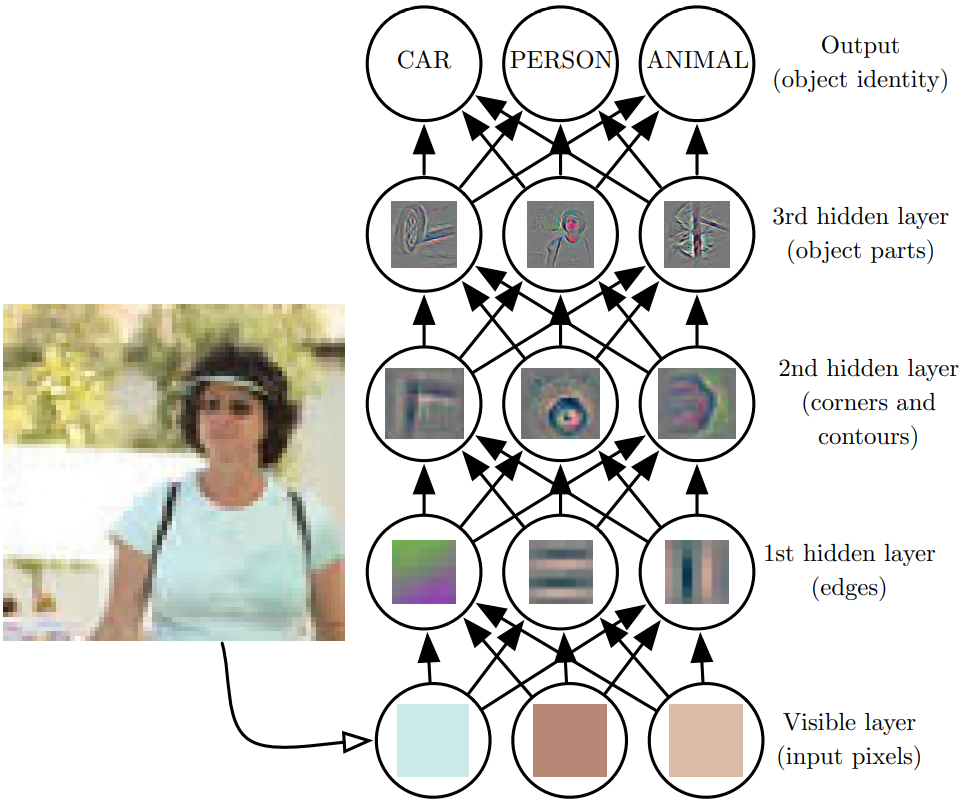
\includegraphics[scale=0.35]{Images/Chapter 6/ffdn-layers.png}
    \caption{Inner workings of a feedforward deep network}
    \source{Goodfellow et al. 2016}
    \label{fig:ch6-innerworkingsofaffdn}
\end{figure}

The idea of learning the right representation for the data provides one perspective on deep learning. A different one is that depth allows the computer to learn a multi-step computer program. Each layer of the representation can be thought of as the state of the computer’s memory after executing another set of instructions in parallel. Networks with greater depth can execute more instructions in sequence. Sequential instructions offer great power because later instructions can refer back to the results of previous ones.

The picture below sums up the differences between various types of artificial intelligence-based systems:

\begin{figure}[hbt]
    \centering
    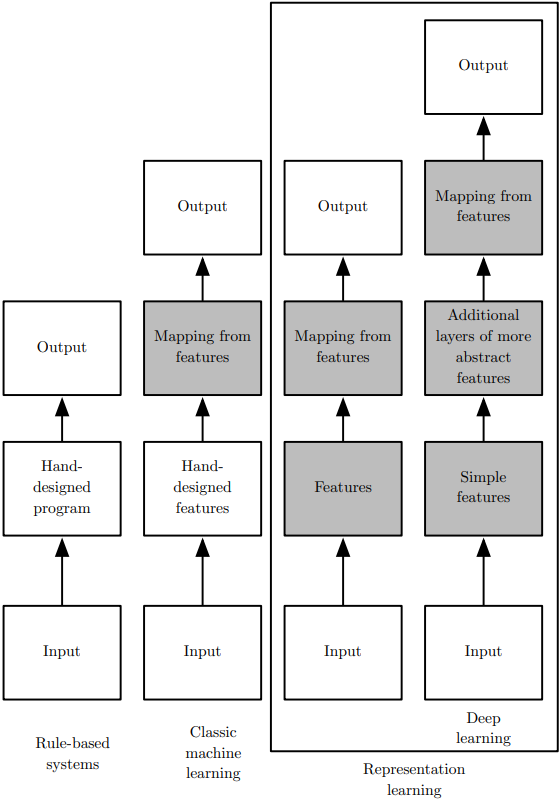
\includegraphics[scale=0.6]{Images/Chapter 6/types-ai.png}
    \caption{Differences between various types of AI-based systems}
    \source{Goodfellow et al. 2016}
    \label{fig:ch6-aitypesdifferences}
\end{figure}

\subsection{From theories of Biological Learning to Deep Learning}
Deep learning only \textit{appears} to be new due to its recent meteoric rise in popularity. As a matter of fact, instead, deep learning has been around since the 1940s, facing alternating periods of fervor and disappointment. There have been three main waves of development of deep learning:

\begin{itemize}
    \item Cybernetics (1940s-1960s).
    \item Connectionism (1980s-1990s).
    \item Deep learning (2006-today).
\end{itemize}

Let us now dive deeper into each of them.

\subsubsection{Cybernetics}
The origins of deep learning go by the name of ``cybernetics'', a term that became widespread thanks to Norbert Weiner’s book ``Cybernetics: control and communication in the animal and machine''. As we can imagine from this title, neuroscience was of great inspiration in this period: some of the earliest learning algorithms, in fact, were intended to be computational models of biological learning, attempting to reproduce what happens (or could happen) in the brain. The brain, in fact, provided a proof by example that intelligent behavior was possible, and a conceptually straightforward path to building intelligence seemed to be to reverse engineer the computational principles behind the brain and to duplicate its functionality. As a result, one of the names that deep learning has gone by is \textbf{artificial neural networks (ANNs)}. This school of thought led to the creation of simple linear models designed to take a set of $n$ input values $x_1,..., x_n$ and associate them with an output $y$. They would then learn a set of weights $w_1,...,w_n$ and compute the output $y=f(\boldsymbol{x},\boldsymbol{w})=x_1 w_1+...+x_n w_n$.

As a brief excursus and to understand the thought process that led to this formulation, we will now spend a few words describing what neurons are and how they work.

Neurons are electrically excitable cells that communicate with other cells via specialized connections called synapses. Communication consists of an all-or-nothing electrochemical pulse (of the same intensity each time the cell is stimulated) that takes place when the voltage of the neuron membrane changes by a large enough amount over a short interval. A typical neuron consists of a cell body (soma), dendrites and a single axon (the latter two being filaments that extrude from the soma) and can be seen in figure \ref{fig:ch6-multipolarneuron}.

\begin{figure}[hbt]
    \centering
    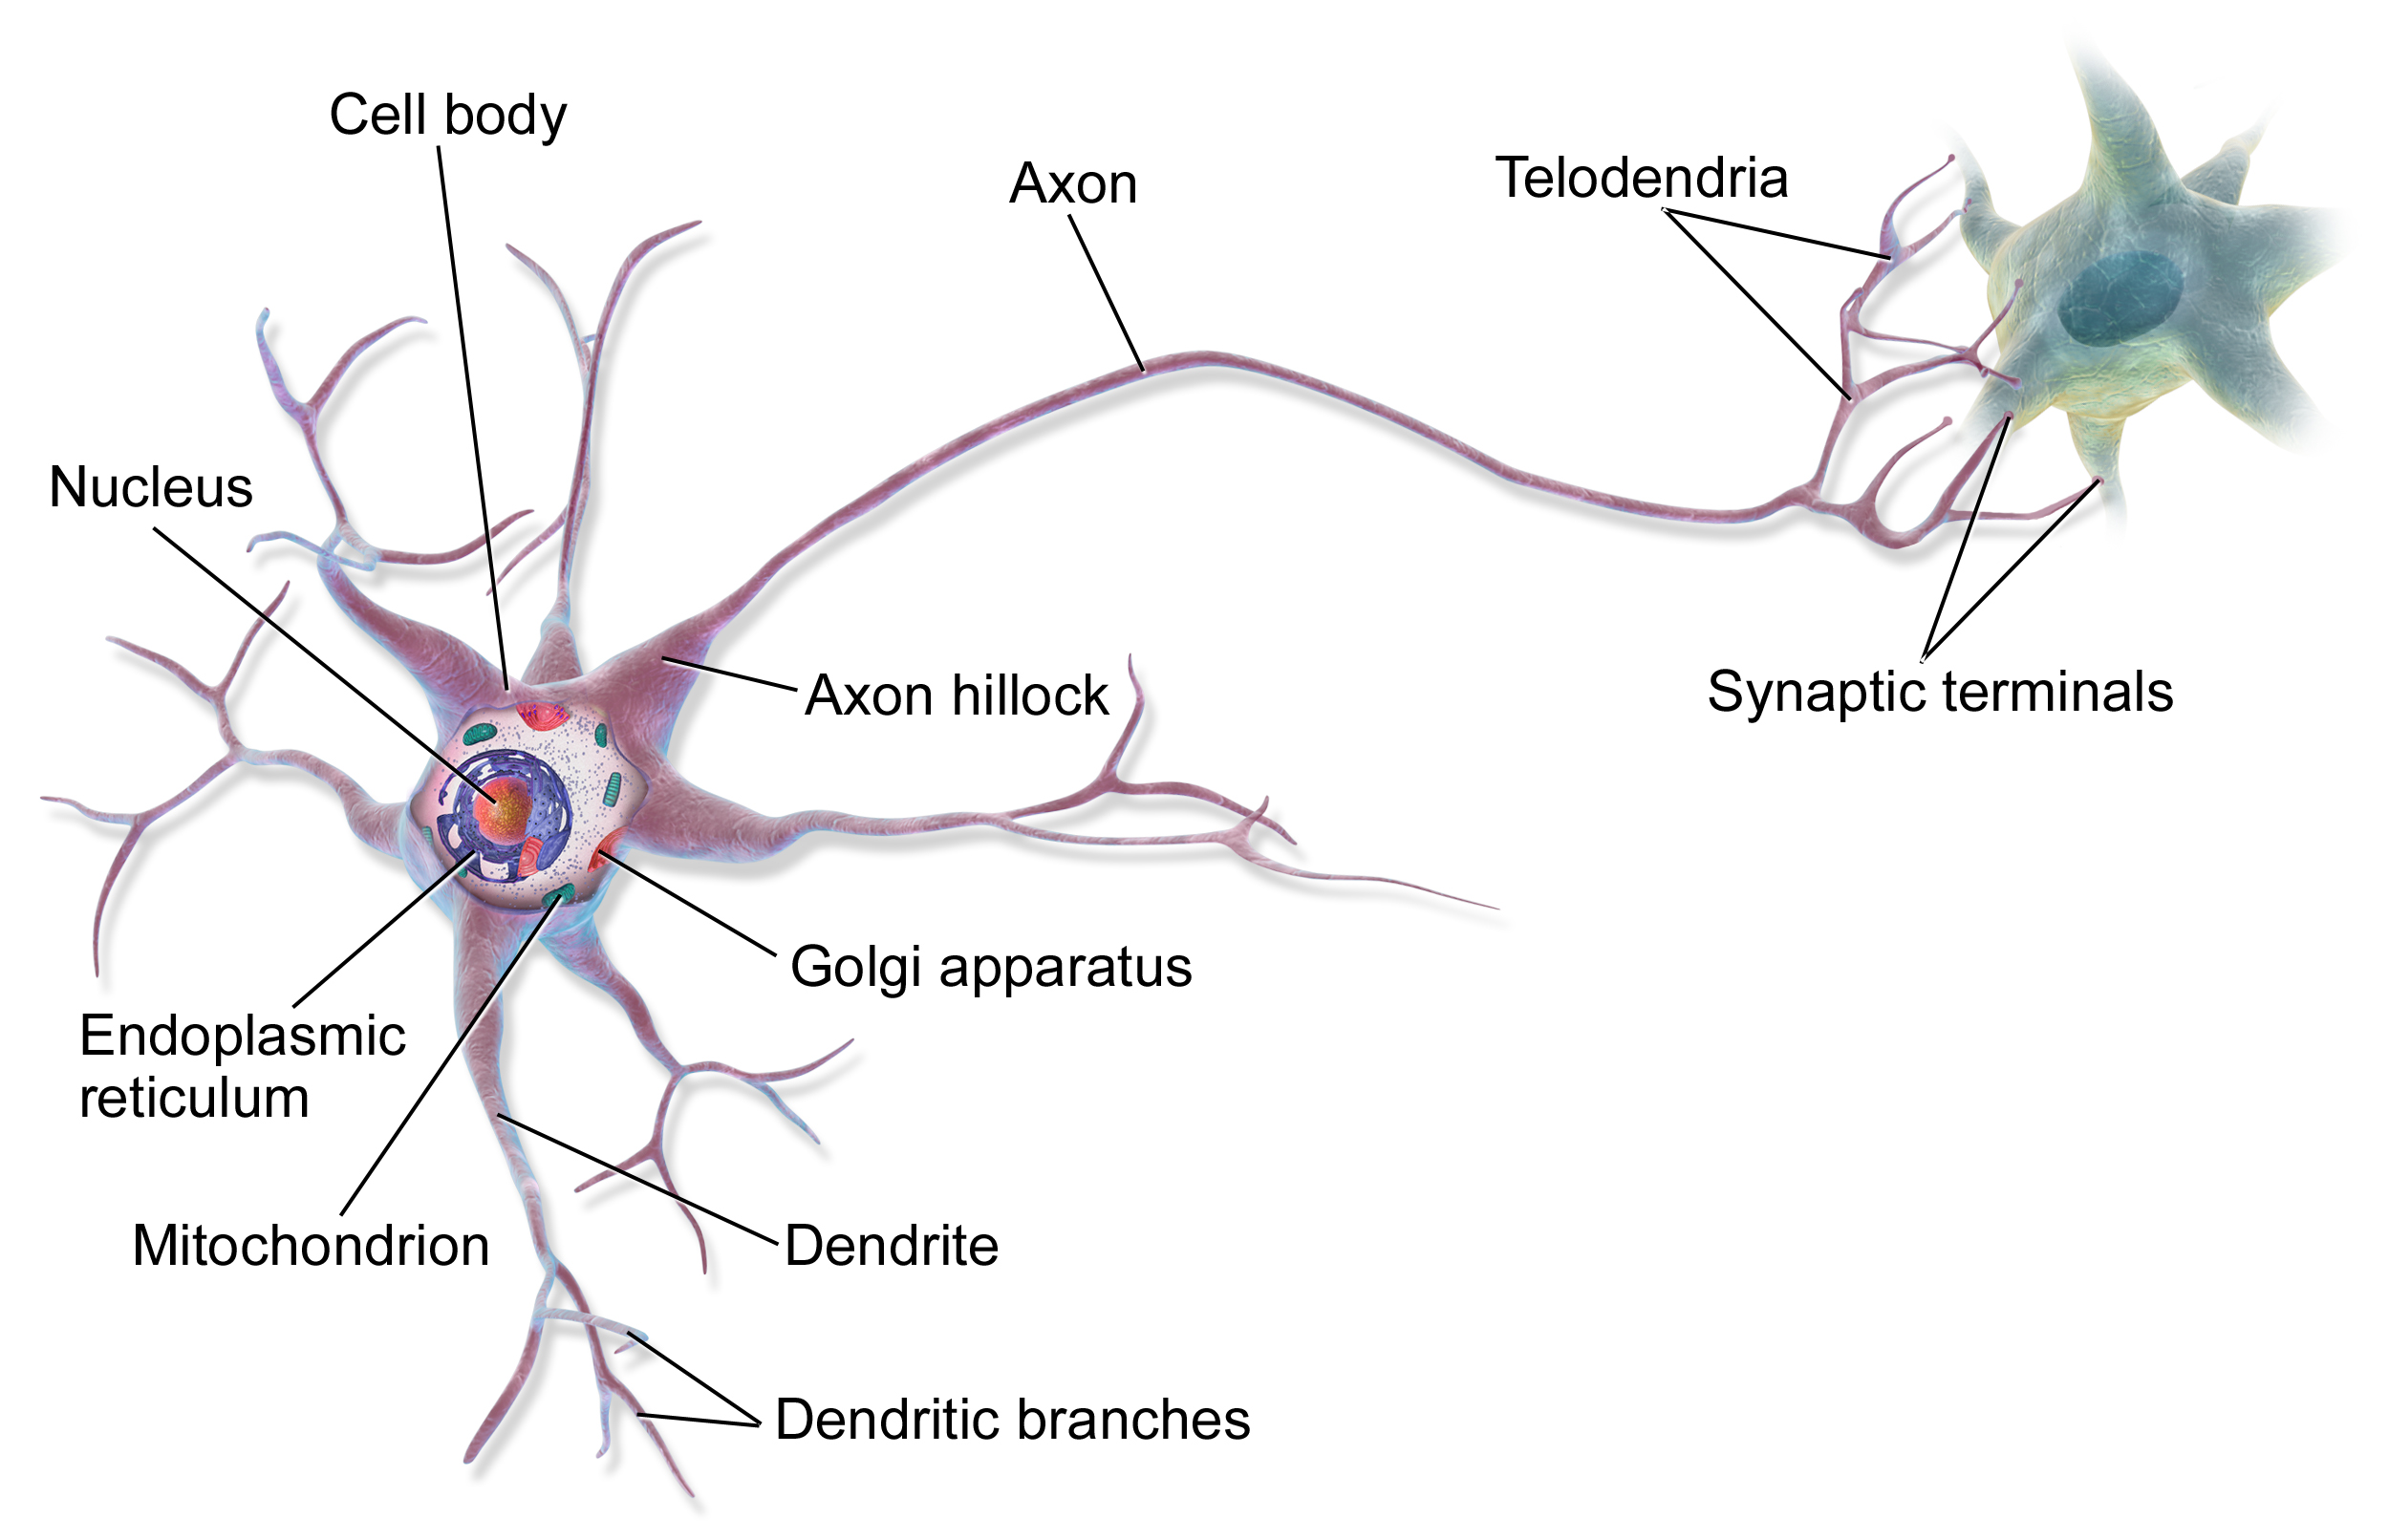
\includegraphics[scale=0.15]{Images/Chapter 6/multipolar neuron.png}
    \caption{Anatomy of a multipolar neuron.}
    \source{BruceBlaus on Wikipedia}
    \label{fig:ch6-multipolarneuron}
\end{figure}

Warren McCulloch (a neuroscientist) and Walter Pitts (a logician) studied the behavior of neurons and concluded that \textit{``Because of the ``all-or-none'' character of nervous activity, neural events and the relations among them can be treated by means of propositional logic''} \cite{MCCULLOCH199099}. In that article they also proposed a model of a simple artificial neuron which output 1 if the weighted sum of the inputs was above a certain threshold and 0 otherwise. Inputs could only have two values, 0 and 1, and be interpreted as \textit{excitatory} or \textit{inhibitory} according to their weights (+1 or -1). This model enabled operations such as \texttt{NOT} (one inhibitory input, with output threshold 0), \texttt{AND} ($n$ excitatory inputs with threshold $n$) and \texttt{OR} ($n$ excitatory inputs with threshold 1) by changing the weights of the inputs. A schema of their model can be found in figure \ref{fig:ch6-mccullochpittsartificialneuron}.

\begin{figure}
    \centering
    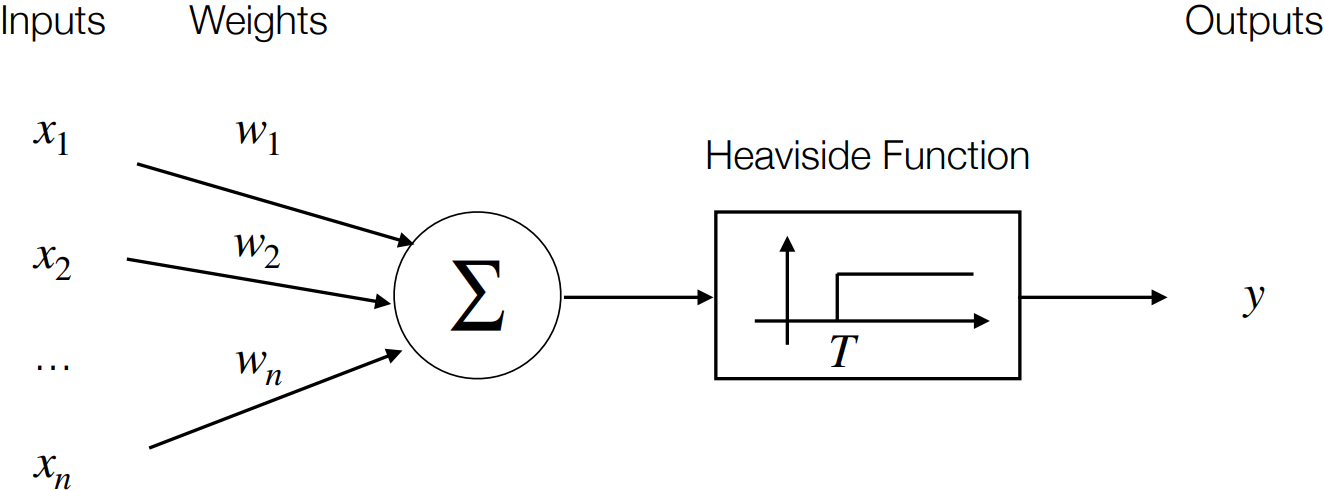
\includegraphics[scale=0.35]{Images/Chapter 6/mcculloch-pitts neuron.png}
    \caption{A schema of McCulloch and Pitt's artificial neuron.}
    \label{fig:ch6-mccullochpittsartificialneuron}
\end{figure}

It is important to note that in their model the weights are \textbf{fixed} and must be set by a human operator. In 1949, though, the neuropsychologist Donald Hebb very importantly pointed out in his book “The Organization of Behavior” that \textit{``When an axon of cell A is near enough to excite a cell B and repeatedly or persistently takes part in firing it, some growth process or metabolic change takes place in one or both cells such that A’s efficiency, as one of the cells firing B, is increased''} \cite{10.1007/978-3-642-70911-1_15}. This means that synaptic connections are reinforced when two or more neurons are activated contiguously in time and space. In simpler words, ``Neurons that fire together, wire together'': the more we do something, the more ``habitual'' that learning will become. Hebb’s model led to the first simulations of artificial neural networks in the 1950s and can be seen in figure \ref{fig:ch6-hebbneuronmodel}.

\begin{figure}
    \centering
    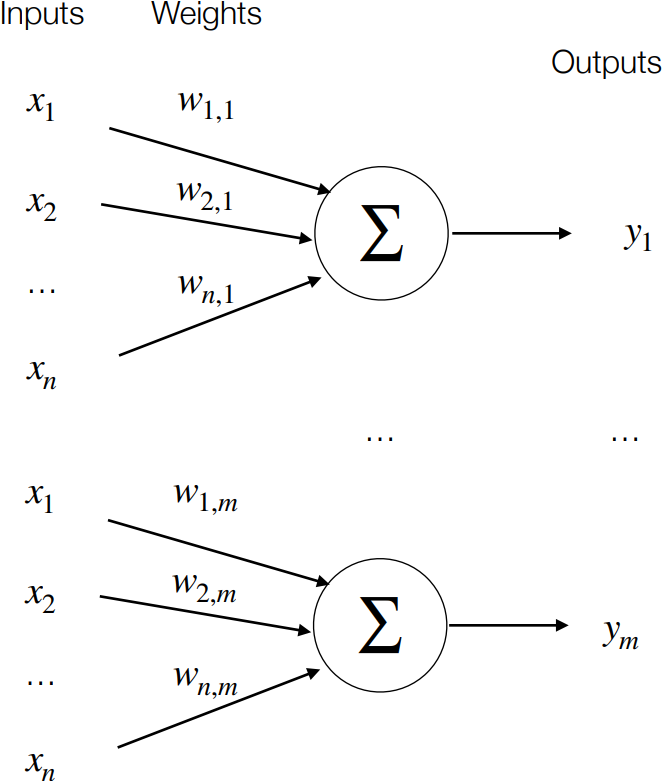
\includegraphics[scale=0.5]{Images/Chapter 6/hebb neuron model.png}
    \caption{Hebb's neuron model}
    \label{fig:ch6-hebbneuronmodel}
\end{figure}

The Hebbian network model has a $n$-node input layer $\boldsymbol{x} = \left[x_1,x_2,...,x_n \right]^T$ and a $m$-node output layer $\boldsymbol{y} = \left[ y_1,y_2, ... ,y_m \right]^T$, with each output being the weighted sum of the corresponding inputs:

\begin{equation*}
    y_i = \sum_{j=1}^{n} w_{j,i} x_j 
\end{equation*}

The strengthening of the connections is represented by the following learning rule:

\begin{equation*}
    w_{j,i}^{new} \leftarrow w_{j,i}^{old} + \eta x_j y_i
\end{equation*}

Where $\eta$ is the \textbf{learning rate}. \emph{It must be noted that this model is different from the way current neural networks work}.

We had to wait until 1958, when Frank Rosenblatt created the \textbf{Perceptron} --a model for a machine that could learn the weights of different categories given examples of those categories-- for these ideas to be put into practice. 

Unfortunately, linear models such as the ones we just presented have many limitations (most famously, they cannot learn the \texttt{XOR} function) and this contributed to a period of disappointment and of little work on this field known as the “AI winter”.

\subsubsection{Connectionism}
The second wave of research on neural networks emerged in the 1980s primarily via a movement called \textbf{connectionism} or \textbf{parallel distributed processing}. Their core idea was that \textbf{many simple computational units could achieve intelligent behavior when networked together}. 

Several key concepts that arose from the connectionist movement remain central to today’s deep learning. Among these we find:

\begin{itemize}
    \item \textbf{Distributed representation}: each concept is not represented by a single neuron, but by a pattern of activation over a large number of neurons. The advantage of distributed representation is that when a small random subset of the network is altered it does not change the macroscopic behavior of the network. However, the disadvantage is that it is hard to interpret or modify the connection strength of the network by an outside observer.
    \item The \textbf{backpropagation algorithm} for training neural networks: the error obtained from the output layer is propagated backwards to the hidden layer and is used to guide training of the weights between the hidden layer and the input layer.
\end{itemize}

Another very important idea that can be found --along with the previous ones-- in a book titled ``Parallel Distributed Processing'' is that of ``Learning and Relearning in Boltzmann Machines'' \cite{10.5555/104279.104291}. A Boltzmann Machine is a network of symmetrically connected, neuron-like units that make stochastic decisions about whether to be on or off based on the data fed to the network while training. We consider two types of Boltzmann Machines, which we can also see in figure \ref{fig:ch6-boltzmannmachines}:

\begin{figure}
    \centering
    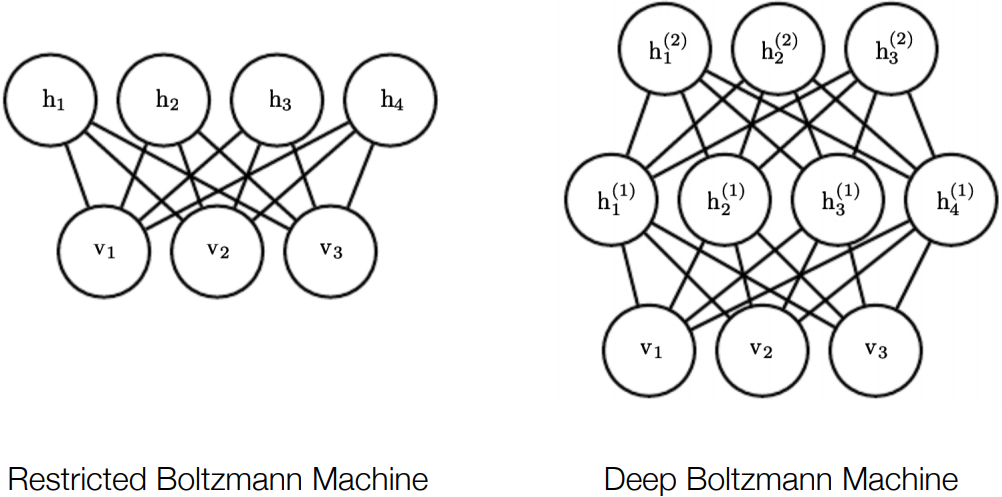
\includegraphics[scale=0.5]{Images/Chapter 6/boltzmann machines.png}
    \caption{Boltzmann machines}
    \label{fig:ch6-boltzmannmachines}
\end{figure}

\begin{itemize}
    \item \textbf{Restricted Boltzmann Machines}, made up of an input and a hidden layer. In this machine neurons must form a bipartite graph\footnote{A graph whose vertices can be divided into two disjoint and independent sets $U$ and $V$ such that every edge connects a vertex in $U$ to one in $V$, see \url{https://en.wikipedia.org/wiki/Bipartite_graph}}.
    \item \textbf{Deep Boltzmann Machines} in which there may be multiple hidden layers, with hidden nodes connected to each other.
\end{itemize}

Note that, unlike most neural networks, the connections are bidirectional and there is no output layer. The training phase for this network leverages the bidirectionality, as it allows for a continuous feedback loop between the input and the hidden layer that is bound to eventually stabilize, allowing the determination of the connection weights. The lack of an output layer is instead explained by the generative nature of these networks: if we give them a partial input (like a section of an image), the network will generate the missing parts, effectively making the results appear in the input layer.

\subsection{Second AI winter and the current AI summer}
The amount of progress being made at the time led to the creation of unrealistic expectations that, once they could not be met, brought in a second AI winter that lasted until the mid-1990s.

The current AI summer, instead, started in 2006, when Geoffrey Hinton and Simon Osindero proposed \textit{``A fast learning algorithm for deep belief nets''}  \cite{10.1162/neco.2006.18.7.1527} (with a strategy called \textit{greedy layer-wise pre-training}) that enabled fast training even for networks with high dimensionality.

This breakthrough opened up a myriad of new possibilities for deep learning. Nowadays, in fact, deep learning applications are aplenty: 

\begin{itemize}
    \item Computer vision.
    \item Machine translation.
    \item Speech generation.
    \item Protein folding.
    \item ...
\end{itemize}

One of deep learning's biggest achievements (and the more relevant one for us) has been its extension to the field of reinforcement learning, enabling what is now known as \textbf{deep reinforcement learning}.
\chapter{Value Function Approximation in Reinforcement Learning}
In this chapter, we will focus on the study of function approximation for estimating state-value functions from on-policy data. That is, approximating $v_\pi$ from experience generated using a known policy $\pi$. The novelty in this chapter is that the approximate value function is not represented as a table, but as a parametrized functional form with a weight vector $\boldsymbol{w} \in \mathbb{R}^d$.

We will write $\hat{v}(s,\boldsymbol{w}) \approx v_\pi (s)$ for the approximate value of state $s$ given a weight vector $\boldsymbol{w}$, with $\hat{v}$ being either a linear function of the weights or, more generally, a (nonlinear) function computed by a multi-layer artificial neural network. Typically, the number of weights is much less than the number of states ($d \ll \left|\mathcal{S}\right|$) and changing one weight changes the estimated value of many states. Consequently, when a single state is updated, the change \textbf{generalizes} from that state to affect the values of many other states. Such generalization makes the learning potentially more powerful, but also potentially more difficult to manage and understand.

In addition to that, if the parametrized function form for $\hat{v}$  does not allow the estimated value to depend on certain aspects of the state, it will behave as if those aspects are unobservable to the agent, making it \textbf{possible to apply these techniques to partially observable problems} as well.

\section{Value function approximation}
Until now, we have seen methods that performed updates to an estimated value function by shifting its value at particular states towards an ``update target'' for that state. Let us refer to an individual update by the notation $s \mapsto u$, where $s$ is the state updated and $u$ is the update target that $s$’s estimated value is shifted towards. For example, the Monte Carlo update for value prediction is $S_t \mapsto G_t$; the TD(0) update is instead $S_t \mapsto R_{t+1} \gamma \hat{v} \left( S_{t+1},\boldsymbol{w}_t \right)$.

It is natural to interpret each update as specifying an example of the desired input-output behavior of the value function. In a sense, the update $s \mapsto u$ means that the estimated value for state $s$ should be more like the update target $u$. If we were to perform this update in tabular methods, we would shift $s$’s estimated value a fraction of the way towards $u$, while leaving the values of the other states unchanged. Now we permit arbitrarily complex and sophisticated methods to implement the update, and updating at $s$ generalizes so that the estimated values of many other states are changed as well. Machine learning methods that learn to mimic input-output examples in this way are called \textbf{supervised learning methods}, and when the outputs are numbers, like $u$, the process is called \textbf{function approximation}.

Artificial neural networks (ANN) are widely used for approximating nonlinear functions, especially because of the guarantees that the \textbf{universal approximation theorem} (initially proven by George Cybenko in 1989) provides. Cybenko, in fact, showed that an ANN with a single hidden layer containing a large enough finite number of sigmoid units can approximate, on a compact region of the network’s input space, any continuous function to any degree of accuracy \cite{Cybenko1989ApproximationBS}.

\section{Stochastic Gradient Descent for function approximation}
We now develop in detail stochastic gradient descent (SGD) methods for function approximation. SGD methods are among the most widely used function approximation methods and are particularly well suited for online reinforcement learning.

To limit the complexity of the matter at hand, we will consider only the case in which we update our network using \textit{only one example at a time}. Let us recall the formula we introduced in the previous chapter for updating the weights using SGD (for batches of examples we can use the mini-batch SGD):

\begin{equation}
    w_j \leftarrow w_j + \Delta w_j = w_j - \eta \frac{\partial J}{\partial w_j}
    \label{eq:ch7-singlesgdupdate}
\end{equation}

Since we will be updating $\boldsymbol{w}$ at each of a series of discrete time steps, $t = 0, 1, 2, ...$, we modify our notation to include the time information as such:

\begin{equation}
    w_{j,t+1} \leftarrow w_{j,t} + \Delta w_{j,t} = w_{j,t} - \eta \frac{\partial J}{\partial w_{j,t}}
    \label{eq:ch7-singlesgdfunctionapproxupdate}
\end{equation}

Assuming that our loss function is represented by the \textbf{mean square error} shown here:

\begin{equation}
    J(\boldsymbol{w}) = \sum_{s \in \mathcal{S}} \big(U_t - \hat{v}(S_t, \boldsymbol{w}_t) \big)^2
    \label{eq:ch7-meansquareerrorfunction}
\end{equation}

--where $U_t$ is our \textbf{target} and $\hat{v}(S_t, \boldsymbol{w}_t)$ is our current estimate-- we will then obtain the following weight update formula:

\begin{equation}
    \begin{split}
        \boldsymbol{w}_{t+1} &\doteq \boldsymbol{w}_t - \frac{1}{2} \eta \nabla \big[ U_t - \hat{v}(S_t, \boldsymbol{w}_t) \big]^2 \\
        &= \boldsymbol{w}_t + \eta \big[ U_t - \hat{v}(S_t, \boldsymbol{w}) \big] \nabla \hat{v} (S_t, \boldsymbol{w}_t)
    \end{split}
    \label{eq:ch7-genericstatefunctionapproxssdweightupdate}
\end{equation}

Since the step-size parameter $\eta$ is chosen arbitrarily, we multiplied it by $\frac{1}{2}$ to cancel out the 2 that comes from the derivative.

\subsection{Semi-gradient one-step SARSA prediction}
The weight update rule we just introduced can be used to extend to state-action value functions the mathematical framework we discussed for state value functions . In this case, the update target $U_t$ will be an approximation of $q_\pi (S_t,A_t )$, making the gradient-descent update as such:

\begin{equation}
    \boldsymbol{w}_{t+1} = \boldsymbol{w}_t + \eta \big[ U_t - \hat{q}(S_t,A_t,\boldsymbol{w}_t) \big] \nabla \hat{q}(S_t,A_t,\boldsymbol{w}_t)
    \label{eq:ch7-genericqvaluefunctionapproxssdweightupdate}
\end{equation}

If we combine this formula with the one we introduced in equation \ref{eq:ch5-sarsaupdaterule}, we obtain the \textbf{episodic semi-gradient one-step SARSA} update rule:

\begin{equation}
    \boldsymbol{w}_{t+1} = \boldsymbol{w}_t + \eta \big[ R_{t+1} + \gamma \hat{q}(S_{t+1},A_{t+1},\boldsymbol{w}_t) - \hat{q}(S_t,A_t,\boldsymbol{w}_t) \big] \nabla \hat{q}(S_t,A_t,\boldsymbol{w}_t)
    \label{eq:ch7-sarsaqvaluefunctionapproxssdweightupdate}
\end{equation}

It is called semi-gradient because we are not really taking the ``real'' gradient, as it would require us to calculate the gradient of $U_t$ as well (simply speaking, we assume the output is not function of $\boldsymbol{w}_t$ even though it is). This is essential to avoid introducing too much complexity and, if the policy is constant, we still have guarantees of convergence.

\subsection{Semi-gradient one-step SARSA control}
As usual, however, we are more interested in the problem of \textit{control}, rather than the one of \textit{prediction}. To tackle it in the case of function approximation, we employ methods that are essentially the same as the ones we used in the tabular case: for each possible action $a$ available in the current state $S_t$, we can compute $\hat{q}(S_t,a,\boldsymbol{w}_t)$ and then find the greedy action using:

\begin{equation*}
    A_{t}^{*} = \argmax_a \hat{q}(S_t,a,\boldsymbol{w}_t)
\end{equation*}

Policy improvement is then done by changing the estimation policy to a soft approximation of the greedy policy (e.g., $\varepsilon$-greedy policy). Since we are in the \textit{on-policy} case, actions are selected according to this same policy. We introduce the pseudo-code for the \textbf{episodic semi-gradient on-policy SARSA algorithm} in the box below:

\begin{algorithm}[H]
\DontPrintSemicolon
\SetAlgoVlined
\KwIn{a differentiable action-value function parametrization $\hat{q}: \mathcal{S} \times \mathcal{A} \times \mathbb{R}^d \rightarrow \mathbb{R}$}
\Parameters{step size $\eta > 0$, small $\varepsilon > 0$}
\Initialize{value-function weights $\boldsymbol{w} \in \mathbb{R}^d$ arbitrarily (e.g., $\boldsymbol{w = 0}$)}

 \Loop{for each episode}{
    $S, A \leftarrow$ initial state and action of episode (e.g., $\varepsilon$-greedy)\;
    \Loop{for each step of the episode}{
        Take action $A$, observe $R, S'$\;
        \If{$S'$ is terminal}{
            $\boldsymbol{w} \leftarrow \boldsymbol{w} + \eta \big[ R - \hat{q}(S,A,\boldsymbol{w})\big] \nabla \hat{q}(S,A,\boldsymbol{w})$\;
            Go to next episode\;
        }
        Choose $A'$ as a function of $\hat{q}(S',\cdot,\boldsymbol{w})$ (e.g., $\varepsilon$-greedy)\;
        $\boldsymbol{w} \leftarrow \boldsymbol{w} + \eta \big[ R + \gamma\hat{q}(S',A',\boldsymbol{w}) - \hat{q}(S,A,\boldsymbol{w})\big] \nabla \hat{q}(S,A,\boldsymbol{w})$\;
        $S \leftarrow S'$\;
        $A \leftarrow A'$\;
    }
 }
\caption{Episodic Semi-gradient SARSA for estimating $\hat{q} \approx q_*$}
\end{algorithm}

\subsection{Semi-gradient off-policy Q-learning}
The same thought process can be applied to obtain \textbf{semi-gradient Q-learning}, in which the update rule will be:

\begin{equation}
    \boldsymbol{w}_{t+1} = \boldsymbol{w}_t + \eta \big[ R_{t+1} + \gamma \argmax_a  \hat{q}(S_{t+1},a,\boldsymbol{w}_t) - \hat{q}(S_t,A_t,\boldsymbol{w}_t) \big] \nabla \hat{q}(S_t,A_t,\boldsymbol{w}_t)
    \label{eq:ch7-qlearningqvaluefunctionapproxssdweightupdate}
\end{equation}

Where $\boldsymbol{w}_t$ is the vector of the network’s weights, $A_t$ is the action selected at time $t$, and $S_t$ and $S_{t+1}$ are the inputs to the network at their respective time steps.

\section{Deep Q-Network}
Semi-gradient Q-learning (or, interchangeably, \textbf{Deep Q-Network}, \textbf{DQN}) has been used to solve Atari games. It combines Q-Learning with a deep (convolutional) neural network, allowing, in this case, the conversion of the original frames from the 60Hz video feed ($210 \times 160$ pixels, 128 colors) in an $84 \times 84$ matrix of luminance values. Since movement is very important in videogames (e.g., what is the direction of the ball in a tennis match, what is its speed, etc.) and it cannot be necessarily inferred from a single frame, researchers decided to feed the network a stack of four frames at a time (making the input $84 \times 84 \times 4$). In addition to that, the rewards of the DQN have been restricted to be one of $\left\{-1,0,+1\right\}$. This has proven to yield better results (possibly) due to a reduction of instability (we learn more quickly if actions that are similar give us the same reward). More information on this can be found in \cite{mnih2013atari} and \cite{mnih2015humanlevel}. Let us now look at some key features of DQN.

We are in the \textbf{control problem}: we want to learn the optimal way to play a game. This, of course, means that the more we learn, the greedier will our policy have to be: once we are confident in our policy, we will have to start playing at the best of our abilities. The value of both $\varepsilon$ and the decay will be part of our \textbf{hyperparameters} and we will have to find their best value experimentally. In the examples cited before, $\varepsilon$ was set to decrease linearly over the first million frames and the network was trained using a mini-batch stochastic gradient with batches of 32 images (each made up of 4 frames), with changes proportional to the running average of the squares of gradients (RMSprop).

Another important thing that may be somewhat counterintuitive, is that the network is made to play all Atari games, and not necessarily any specific one: the output layer (as shown in figure \ref{fig:ch7-dqnschema}) will then always be made up of 18 nodes, even though only a subset may ever have values that are not 0.

\begin{figure}
    \centering
    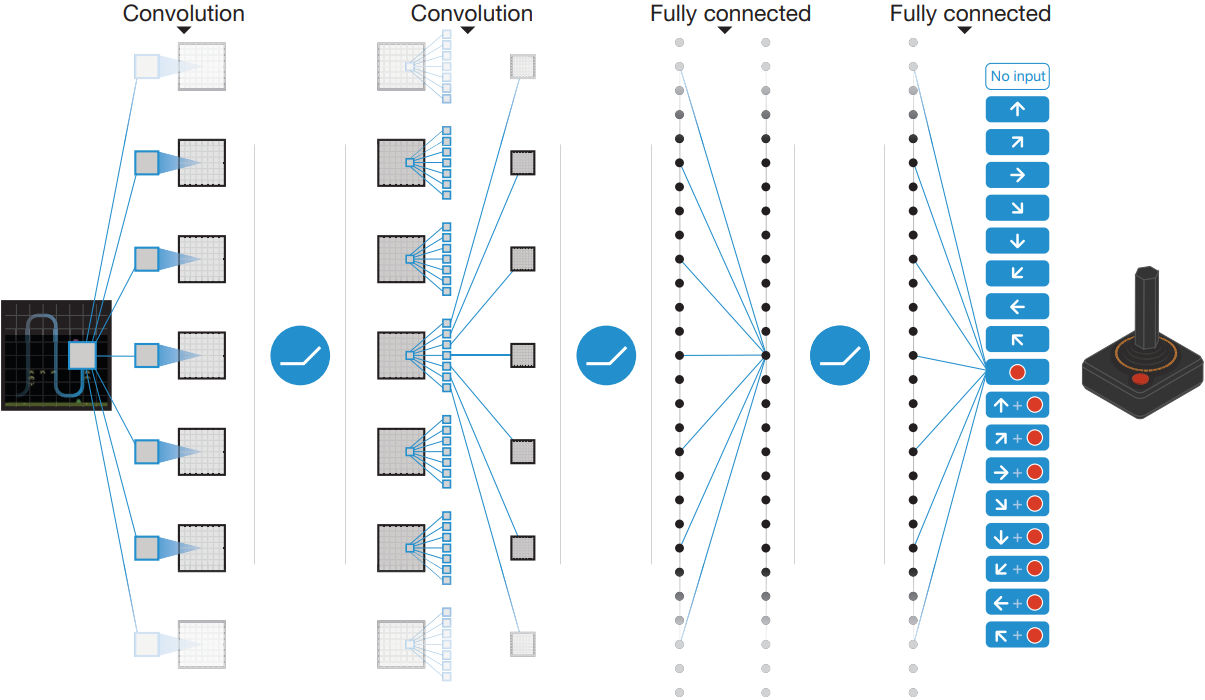
\includegraphics[scale=0.4]{Images/Chapter 7/ataridqn.png}
    \caption{DQN Schema}
    \source{Mnih et al. 2013}
    \label{fig:ch7-dqnschema}
\end{figure}

The authors of DQN made a series of changes to the ``standard'' Q-learning, the most important of which has probably been the introduction of \textbf{experience replay} to deal with the convergence problem of Q-learning. Picking actions that are highly correlated, in fact, has the effect of limiting our exploration of the space, thus leading to a much slower process of convergence (e.g., we may learn to run well on tarmac, but as soon as we go on sand, it will take us quite a while to adapt, causing updates with \textbf{high variance} to compensate).

The key idea is then to perform training through an \textbf{emulator} and storing the agent’s experience in a \textbf{replay memory} that is accessed to perform the weight updates. In practice, after the emulator executes action $A_t$ in a state represented by the image stack $S_t$, receiving reward $R_{t+1}$, we add to the replay memory (or \textbf{replay buffer}) a tuple made up of these values and the image stack $S_{t+1}$: $\big(S_t,A_t,R_{t+1},S_{t+1}\big)$. Each Q-learning update will then be performed by randomly sampling from the experience replay buffer. Instead of $S_{t+1}$ becoming the new $S_t$ for the next update, as it happens in normal Q-learning, a new, unconnected experience is drawn from the replay memory, helping us avoid getting stuck with actions that do not generalize. It is important to note that this is possible because Q-learning is an \textit{off-policy} algorithm, and so it does not need to learn from ``connected'' trajectories. More information can be found in \cite{10.1007/BF00992699}.
\chapter{Policy Gradient Methods}
Until now we have discussed so-called \textbf{action-value methods}, in which we learn the action values and use a policy (e.g., $\varepsilon$-greedy) to select actions based on those estimates. A possible alternative would be to have a different set of methods that could learn a \textbf{parametrized policy that allowed them to select actions without consulting a value function} (a value function might be used to learn the policy parameter, but it is not required for action selection; we will keep using the $\boldsymbol{w} \in \mathbb{R}^d$ notation for the weight vector of the value function).

For \textbf{policy networks} we will use $\boldsymbol{\theta}$ to indicate the \textbf{policy’s parameter vector}, with $\boldsymbol{\theta} \in \mathbb{R}^{d'}$. The probability of taking an action $a$ at time $t$, given that the environment is in state $s$ at time $t$ with parameter $\boldsymbol{\theta}$, will then be:

\begin{equation*}
    \pi \left( a \middle\vert s, \boldsymbol{\theta} \right) = \text{Pr}\left\{ A_t = a \ \middle\vert \ S_t = s, \boldsymbol{\theta}_t = \boldsymbol{\theta} \right\}
\end{equation*}

The methods that will be introduced in this chapter will learn the policy parameter $\boldsymbol{\theta}$ by means of (the gradient of) a scalar performance measure $J(\boldsymbol{\theta})$. Since these methods will seek to \textit{maximize} performance\footnote{Earlier we were trying to \textbf{minimize the error} in the Q-value estimation, whereas now we are trying to \textbf{maximize the performance} of our policy.}, their updates will work towards approximating \textbf{gradient ascent} in $J$:

\begin{equation}
    \boldsymbol{\theta}_{t+1} = \boldsymbol{\theta}_t + \alpha \widehat{\nabla J(\boldsymbol{\theta}_t)}
    \label{eq:ch8-gradientascentupdate}
\end{equation}

Where $\widehat{\nabla J(\boldsymbol{\theta}_t)} \in \mathbb{R}^{d'}$ is a stochastic estimate whose expectation approximates the gradient of the performance measure with respect to its argument $\boldsymbol{\theta}_t$. In simpler terms, we perform our weight correction in the direction that, based on our estimate of $J(\boldsymbol{\theta})$, will lead to a gradient ascent. Methods that follow this schema are called \textbf{policy gradient methods}.

\section{Policy approximation and its advantages}
In policy gradient methods, the policy can be parametrized in any way, with one caveat: $\pi \left( a \middle\vert s, \boldsymbol{\theta} \right)$ must be differentiable with respect to its parameters, that is, as long as $\nabla \pi \left( a \middle\vert s, \boldsymbol{\theta} \right)$ exists and is finite $\forall s \in \mathcal{S}, a \in \mathcal{A}(s)$ and $\boldsymbol{\theta} \in \mathbb{R}^{d'}$. In practice, however, to ensure exploration it is usually required that the policy never becomes deterministic.

A common way to parametrize policies is to form a \textbf{parametrized numerical preference} $h(s,a,\boldsymbol{\theta}) \in \mathbb{R}$ for each state-action pair (this is often the case when the action space is discrete and not too large). The actions with the highest preferences in each state will then be given the highest probabilities of being selected, typically according to an exponential soft-max distribution as such:

\begin{equation}
    \pi \left(a \middle\vert s, \boldsymbol{\theta} \right) \doteq \frac{e^{h(s,a,\boldsymbol{\theta})}}{\sum_{b} h(s,b,\boldsymbol{\theta})}
    \label{eq:ch8-softmaxinactionpreferencesparametrization}
\end{equation}

Where $e \approx 2.71828$ is Euler’s number, the base of the natural logarithm. This type of policy parametrization is called \textbf{soft-max in action preferences}.

The parametrization of the action preferences is arbitrary, too. The $h(s,a,\boldsymbol{\theta}) \in \mathbb{R}$ values might be computed, for example, by a deep artificial neural network, where $\boldsymbol{\theta}$ is the vector of all the connection weights of the network (like in the case of AlphaGo). This is just one of the options, but it helps us scale up.

One advantage of parametrizing policies according to the \textit{soft-max in action preferences} is that the approximate policy can approach a deterministic one, whereas with $\varepsilon$-greedy we would always have an $\varepsilon$ probability of selecting a random action. We could also select actions according to a soft-max distribution based on action values, but this alone would not allow the policy to approach a deterministic one. The action-value estimates would end up converging to their true values, which would differ by a finite amount, causing the soft-max function to output specific probabilities, and not just 0 and 1. Action preferences are different because they \textit{do not approach specific values}; instead, \textit{they are driven to produce the optimal stochastic policy}: if the optimal policy is deterministic, then the preferences of the optimal actions will be driven infinitely higher than all suboptimal actions (if permitted by the parametrization).

A second advantage is that this method enables the selection of actions with arbitrary probabilities. This means that, when dealing with problems where the best approximate policy is stochastic (such as in rock-paper-scissors), we can even learn to choose one of the available actions with equal probability, something that is not possible with action-value methods.

Last, and perhaps the simplest, advantage that policy parametrization may have over action-value parametrization is that the policy may be a simpler function to approximate, converging faster and more smoothly.

\section{Policy Gradient Theorem}
As we just said, with continuous policy parametrization the action probabilities change smoothly as a function of the learned parameter, whereas in $\varepsilon$-greedy selection the action probabilities may change dramatically for an arbitrary small change in the estimated action values, if that change results in a different action having the maximal value. Largely because of this, policy gradient methods have stronger convergence guarantees compared to action-value methods.

Let us consider \textbf{episodic learning}, for which we define the performance measure as the value of the start state of the episode\footnote{Our objective is to play to the best of our abilities, which means maximizing the expected cumulative rewards $G$. We obtain exactly that by maximizing the value of the initial state.}. We simplify the notation (without losing any meaningful generality) by assuming that every episode starts in some particular (non-random) state $s_0$. The performance is then defined as:

\begin{equation*}
    J(\boldsymbol{\theta}) \doteq v_{\pi_{\boldsymbol{\theta}}}(s_0)
\end{equation*}

Where $v_{\pi_{\boldsymbol{\theta}}}$ is the true value function for $\pi_{\boldsymbol{\theta}}$, the policy determined by $\boldsymbol{\theta}$. The issue now becomes how to change the policy parameter $\boldsymbol{\theta}$ by means of function approximation in a way that ensures improvement.

Doing so is more complicated than it may seem from a superficial look. Performance --as in, how good our policy is-- depends on two things:

\begin{itemize}
    \item The actions we choose in a certain state.
    \item The states that the policy makes us go through.
\end{itemize}

Both factors are affected by the policy parameter. However, while it is easy to compute, given a state and knowledge of the parametrization, the effect of the policy parameter on the actions, the effect of the policy on the state distribution (the states that we end up visiting) is a function of the environment, which is typically unknown, making it impossible to estimate. 

How can we then perform gradient ascent (formula \ref{eq:ch8-gradientascentupdate}) if the gradient of the performance with respect to the policy parameter depends on the unknown effect of policy changes on the state distribution?  The \textbf{policy gradient theorem} comes to our rescue, providing us with an analytic expression of the gradient that does not involve the derivative of the state distribution, as we can see below:

\begin{equation}
    \nabla J(\boldsymbol{\theta}) \propto \sum_s \mu(s) \sum_a q_\pi(s,a) \nabla\pi(a \vert s, \boldsymbol{\theta})
    \label{eq:ch8-policygradienttheorem}
\end{equation}

Where the gradients are column vectors of partial derivatives with respect to the components of $\boldsymbol{\theta}$ and $\pi$ denotes the policy corresponding to parameter vector $\boldsymbol{\theta}$. $\mu(s)$ is the \textbf{on-policy distribution} under policy $\pi$ and it describes the normalized frequency with which states are encountered while the agent is selecting actions according to $\pi$ or, to put it differently, it is the normalized fraction of time spent in each state. A proof for this formula can be found in Sutton and Barto’s book on page 325.

We might then ask: the policy gradient theorem only provides us with something that is \textit{proportionate to} the gradient, and not \textit{equal to}, does it still work? The answer is yes, in the weight update formula, in fact, we can use the step size $\alpha$ to turn this proportionality into an equality by setting it to the average length of an episode.

\section{REINFORCE: Monte Carlo Policy Gradient}
As we mentioned in the beginning of this chapter, our strategy of stochastic gradient ascent is based on $\widehat{\nabla J(\boldsymbol{\theta}_t)}$, a stochastic estimate whose expectation approximates the gradient of the performance measure with respect to its argument $\boldsymbol{\theta}_t$. Thanks to the policy gradient theorem, this approximation is sufficient, and we can ``absorb'' the error of this estimate in the step size constant $\alpha$. 

The problem at hand now becomes finding a way of sampling whose expectation equals or approximates the expression given by the policy gradient theorem\footnote{Since the update formula is based on $\widehat{\nabla J(\boldsymbol{\theta}_t)}$, a stochastic estimate of the gradient of the performance function with respect to its parameters, we need to find a way to sample $\nabla J(\boldsymbol{\theta})$. We do so by applying the policy gradient theorem.}. Given the definition of $\mu$ we gave earlier, we can see the right-hand side of the theorem as a sum over states weighted by how often the state occurs under the target policy $\pi$. If $\pi$ is followed, then the states will be encountered in these proportions, which means that:

\begin{equation}
    \begin{split}
        \nabla J(\boldsymbol{\theta}) &\propto \sum_s \mu(s) \sum_a q_\pi(s,a) \nabla\pi(a \vert s, \boldsymbol{\theta}) \\
        &= \mathbb{E}_\pi \Bigg[ \sum_a q_\pi (S_t, a) \nabla \pi (a \vert S_t, \boldsymbol{\theta}) \Bigg]
    \end{split}
    \label{eq:ch8-statesampledpolicygradient}
\end{equation}

As a reminder, we defined $\mathbb{E}_\pi \left[\cdot\right]$ as the expected value of a random variable given that the agent follows $\pi$.

In theory, we could stop here and instantiate the stochastic gradient-ascent algorithm (\ref{eq:ch8-gradientascentupdate}) as:

\begin{equation*}
    \boldsymbol{\theta}_{t+1} \doteq \boldsymbol{\theta}_{t} + \alpha \sum_a \hat{q}(S_t,a,\boldsymbol{w}) \nabla \pi (a \vert S_t, \boldsymbol{\theta})
\end{equation*}

Where $\hat{q}$ is some learned approximation of $q_\pi$. We obtained an \textbf{all-action method}, because its update involves all the actions in each update, but our focus is on REINFORCE, whose update at time $t$ involves just $A_t$, the action actually taken at time $t$.

We continue our derivation of REINFORCE by introducing $A_t$ in the same way we introduced $S_t$ just now: by replacing a sum over the random variable’s possible values by an expectation under $\pi$ and then sampling the expectation. Equation \ref{eq:ch8-statesampledpolicygradient} now becomes:

\begin{equation}
    \begin{split}
        \nabla J(\boldsymbol{\theta}) &\propto \mathbb{E}_\pi \Bigg[ \sum_a q_\pi (S_t, a) \nabla \pi (a \vert S_t, \boldsymbol{\theta}) \Bigg] \\
        &= \mathbb{E}_\pi \Bigg[ \sum_a \pi (a \vert S_t, \boldsymbol{\theta}) \cdot q_\pi (S_t, a) \nabla \pi (a \vert S_t, \boldsymbol{\theta}) \cdot \frac{1}{\pi (a \vert S_t, \boldsymbol{\theta})} \Bigg] \\
        &= \mathbb{E}_\pi \Bigg[ \mathbb{E}_\pi \left[ q_\pi (S_t, A_t) \right] \frac{\nabla \pi (a \vert S_t, \boldsymbol{\theta})}{\pi (a \vert S_t, \boldsymbol{\theta})} \Bigg] \quad \text{since } \mathbb{E}_\pi \left[\mathbb{E}_\pi[\cdot]\right] = \mathbb{E}_\pi [\cdot] \\
        &= \mathbb{E}_\pi \Bigg[ q_\pi (S_t, A_t) \frac{\nabla \pi (a \vert S_t, \boldsymbol{\theta})}{\pi (a \vert S_t, \boldsymbol{\theta})} \Bigg] \quad \text{since } \mathbb{E}_\pi \left[G_t \vert S_t, A_t \right] = q_\pi (S_t, A_t) \\
        &= \mathbb{E}_\pi \Bigg[ G_t \frac{\nabla \pi (a \vert S_t, \boldsymbol{\theta})}{\pi (a \vert S_t, \boldsymbol{\theta})} \Bigg]
    \end{split}
    \label{eq:ch8-stateandactionsampledpolicygradient}
\end{equation}

We now have an expression that can be sampled on each time step and whose expectation is proportional to the gradient. Using this sample to instantiate our generic stochastic gradient ascent algorithm, we obtain the REINFORCE update rule:

\begin{equation}
    \boldsymbol{\theta}_{t+1} \doteq \boldsymbol{\theta}_{t} + \alpha G_t \frac{\nabla \pi (a \vert S_t, \boldsymbol{\theta})}{\pi (a \vert S_t, \boldsymbol{\theta})}
    \label{eq:ch8-reinforceupdaterule}
\end{equation}

With this rule, each increment is proportional to the product of a return $G_t$ and a vector, the gradient of the probability of taking the action actually taken divided by the probability of taking that action. The vector is the direction in the parameter space that most increases the probability of repeating the action $A_t$ on future visits to state $S_t$. The update increases the parameter vector in this direction proportional to the return, and inversely proportional to the action probability. The former makes sense because it causes the parameter to move most in the directions that favor actions that yield the highest return. The latter makes sense because otherwise actions that are selected frequently are at an advantage (the updates will be more often in their direction) and might win out even if they do not yield the highest return.

If we then apply the identity $\nabla \ln{x} = \frac{\nabla x}{x}$, we obtain the final formulas:

\begin{equation}
    \nabla J(\boldsymbol{\theta}) \propto \mathbb{E}_\pi \Big[ G_t \nabla \ln{\pi (a \vert S_t, \boldsymbol{\theta})} \Big]
    \label{eq:ch8-finalreinforcepolicygradient}
\end{equation}

\begin{equation}
    \boldsymbol{\theta}_{t+1} \doteq \boldsymbol{\theta}_{t} + \alpha G_t \nabla \ln{\pi (a \vert S_t, \boldsymbol{\theta})}
    \label{eq:ch8-finalreinforceupdaterule}
\end{equation}

A pseudocode implementation of REINFORCE is provided here:

\begin{algorithm}[H]
\DontPrintSemicolon
\SetAlgoVlined
\KwIn{a differentiable policy parametrization $\pi (a \vert S_t, \boldsymbol{\theta})$}
\Parameters{step size $\alpha > 0$}
\Initialize{policy parameter $\boldsymbol{\theta} \in \mathbb{R}^{d'}$ (e.g., to $\boldsymbol{0}$)}

 \Loop{for each episode}{
    Generate an episode $S_0, A_0, R_1, ..., S_{T-1}, A_{T-1}, R_T$, following $\pi(\cdot \vert \cdot, \boldsymbol{\theta})$\;
    \Loop{for each step of the episode $t = 0, 1, ..., T-1$}{
        $G \leftarrow \sum_{k = t+1}^{T} R_k$\;
        $\boldsymbol{\theta} \leftarrow \boldsymbol{\theta} + \alpha G \nabla \ln{\pi (A_t \vert S_t, \boldsymbol{\theta})}$
    }
 }
\caption{REINFORCE: Monte-Carlo Policy-Gradient Control (episodic) for $\pi_*$}
\end{algorithm}

To have a better idea of how this is could be put into practice in a neural network, we can look at figure \ref{fig:ch8-reinforcepolicynetwork}.

\begin{figure}[hbp]
    \centering
    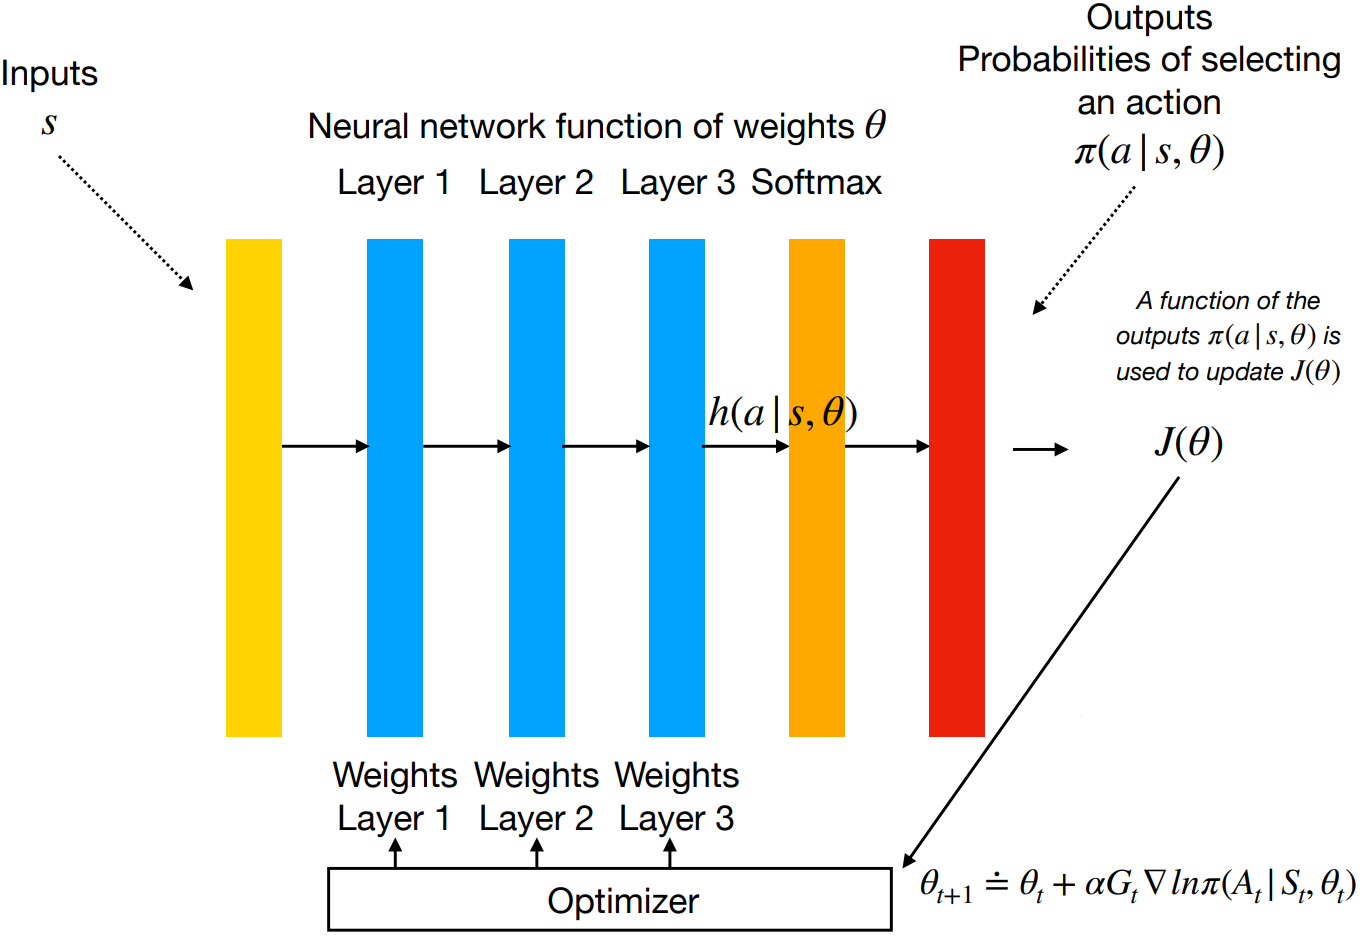
\includegraphics[scale=0.35]{Images/Chapter 8/reinforce-policy-network.png}
    \caption{A neural network using REINFORCE}
    \source{Prof. Mirco Musolesi}
    \label{fig:ch8-reinforcepolicynetwork}
\end{figure}

\section{Stochastic Gradient Ascent}
What we have seen in picture \ref{fig:ch8-reinforcepolicynetwork} works, except for one not-so-minor detail: neural networks (and the backpropagation algorithm) work by minimizing the loss function, performing stochastic gradient \textit{descent}, which is the opposite of what we want to do (an explanation of how stochastic gradient descent works can be found in \autoref{subsection:gradient-based-optimization}).

A simple --but effective-- trick to have neural networks perform stochastic gradient \textit{ascent} is then to have a new function $J' (\boldsymbol{\theta})$ that is the opposite of $J(\boldsymbol{\theta})$. Formally, we will have:

\begin{itemize}
    \item $J' (\boldsymbol{\theta}) = -(G_t \ln{\pi} - 0) = -G_t \ln{\pi}$
    \item $\nabla J' (\boldsymbol{\theta}) = -G_t \nabla \ln{\pi}$
\end{itemize}

\chapter{Multiagent learning}
Until now we have been studying situations in which only one autonomous agent was present in the environment, learning how it could be trained to act in optimal ways. Often, however, there may be multiple agents in the same environment, interacting with each other and learning. This will be the focus of this chapter.

Let us start with two definitions of multiagent systems:

\begin{itemize}
    \item \textit{``Multiagent systems are distributed systems of independent actors called agents that are independently controlled but that interact with one another in the same environment''}. \cite{wooldridge02} \cite{10.1007/978-3-030-01713-2_1}
    \item \textit{``Multiagent systems are systems that include multiple autonomous entities with (possibly) diverging information''}. \cite{ShohamLeytonBrown09}
\end{itemize}

These definitions highlight a few very important characteristics of multiagent systems:

\begin{itemize}
    \item Each agent is \textit{independent} and has its own ``brain'', a (possibly) totally different piece of software controlling the agent.
    \item Agents can take actions in the environment, possibly changing it for the rest of the agents.
    \item Each agent may have a limited -and different, possibly even diverging- view of the environment.
\end{itemize}

Our focus will be the case in which the behavior of the agents is not hardwired, but it can be changed and improved over time towards a goal. Our definition of multiagent learning will then be \textit{``the study of multiagent systems in which one or more of the autonomous entities improves automatically through experience''}.

It is not difficult to imagine how different characteristics of the environment and of the agents might play a role in the overall complexity of the system. As an example, we might consider different scales of environments (such as a city, an ant colony, or a football team) and agents with different degrees of complexity (like a human, a machine, or an insect). A particularly hot topic of research in the field of multiagent systems is cooperation and trust among agents. An agent set in a city, for example, might give less importance to ``behaving well'' compared to one set in a small village, as it tends to interact with different agents each time (it does not necessarily need to establish relationships based on trust).

Possibly the most important feature that a system should have to allow agents to learn is \textbf{regularity}. To learn, in fact, we must have something that does not change drastically over time, something that can be relied upon to implement a strategy. We will make the assumption that past experience is somehow predictive of future expectations (dealing with non-stationarity is another topic of current research).

In this chapter we will consider five paradigms:

\begin{itemize}
    \item Online multi-agent reinforcement learning towards an individual utility.
    \item Online multi-agent reinforcement learning towards social welfare.
    \item Co-evolutionary learning.
    \item Swarm intelligence.
    \item Adaptive mechanism design.
\end{itemize}

\section{Online RL towards individual utility}
One of the most studied scenarios in multiagent learning is that in which multiple independent agents take actions in the same environment and learn online to maximize their own utility function.

From a formal point of view (leveraging game theory), this can be considered a \textbf{repeated normal-form game}. It is repeated because it is based on a certain number of repetitions and normal form because it is represented by means of a matrix\footnote{More can be found on Wikipedia: \url{https://en.wikipedia.org/wiki/Repeated_game} \url{https://en.wikipedia.org/wiki/Normal-form_game}}.

\subsection{(Repeated) Normal-form games}
To better understand normal-form games, we introduce the \textit{``Prisoner’s dilemma''}, a standard example of a game analyzed in game theory that shows why two completely rational individuals might not cooperate, even if it appears that it is in their best interests to do so

The game is as such: two members of a criminal gang are arrested and imprisoned. Each prisoner is in solitary confinement with no means of communicating with the other. The prosecutors lack sufficient evidence to convict the pair on the principal charge, but they have enough to convict both on a lesser charge. Simultaneously, the prosecutors offer each prisoner a bargain. Each prisoner is given the opportunity either to betray the other by testifying that the other committed the crime, or to cooperate with the other by remaining silent. The possible outcomes are:

\begin{itemize}
    \item If the two prisoners remain silent (they \textbf{cooperate}), they will both serve one year in prison (corresponding to a payoff of 2).
    \item If A betrays B (A \textbf{defects}), A will be set free (payoff of 3), and B will serve 3 years in prison (payoff of 0).
    \item If the prisoners betray each other, they will both serve two years in prison (with a payoff of 1)\footnote{Adapted from \url{https://en.wikipedia.org/wiki/Prisoner\%27s_dilemma}}.
\end{itemize}

Since it is a normal-form game, we can represent it in a matrix:

\noindent\begin{minipage}{\linewidth}
\centering
\arrayrulecolor{black}
\begin{tabular}{!{\color{black}\vrule}l!{\color{black}\vrule}c!{\color{black}\vrule}c!{\color{black}\vrule}} 
\hline
~         & \multicolumn{1}{l!{\color{black}\vrule}}{Defect} & \multicolumn{1}{l!{\color{black}\vrule}}{Cooperate}  \\ 
\hline
Defect    & (1,1)                                            & (3,0)                                                \\ 
\hline
Cooperate & (0,3)                                            & (2,2)                                                \\
\hline
\end{tabular}
\arrayrulecolor{black}
\end{minipage}

These types of games were initially introduced as one-shot games, where the players knew each other’s reward functions and play the game only once. In this setting, the concept of Nash equilibrium was introduced: a set of actions such that no player has anything to gain from changing their strategy, assuming that the opponent’s strategy is fixed. Games can have one or multiple Nash equilibria. In the case of the prisoner’s dilemma, the only equilibrium is for both agents to defect.

In the case of repeated normal-form games, players interact with one another multiple times, with the objective of maximizing their expected returns over time.

\section{Online RL towards social welfare}
An alternative paradigm to the one just presented is one in which multiple independent agents take actions in the same environment and learn online to maximize a global utility function. These are also called coordination games, where different players coordinate to achieve a given objective (e.g., maximize the global expected return).

An application of this can be seen in the ``Multiagent Cooperation and Competition with Deep Reinforcement Learning'' paper by Tampuu et al. \cite{DBLP:journals/corr/TampuuMKKKAAV15} where two agents learn how to play Pong in a way that maximizes the length of the game, making sure none of the two players lose. To achieve this, the agents learn techniques such as not serving the ball or bouncing it in a straight line, as depicted in the image below.

\begin{figure}
    \centering
    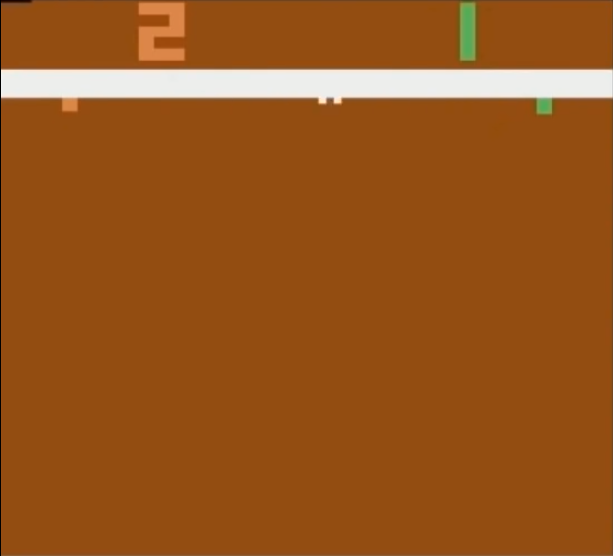
\includegraphics[scale=0.35]{Images/Chapter 9/multiagent-pong.png}
    \caption{Pong being played by two agents}
    \source{Computational Neuroscience Lab at University of Tartu on YouTube}
    \label{fig:ch9-multiagentpong}
\end{figure}

\section{Co-evolutionary approaches}
Evolution can also be used to model and learn agent behavior as well. According to this paradigm, abstract Darwinian models of evolution are applied to refine populations of agents (known as \textit{individuals}) over generations by means of \textbf{evolutionary algorithms}. 

Evolutionary algorithms are made up of five steps\footnote{More can be read on \url{https://towardsdatascience.com/introduction-to-genetic-algorithms-including-example-code-e396e98d8bf3} and \url{https://en.wikipedia.org/wiki/Evolutionary_algorithm}}:

\begin{itemize}
    \item Creation of the initial population by randomly generating agents. Each agent is characterized by a set of parameters called \textbf{genes} (that are joined into strings called \textbf{chromosomes}).
    \item Calculation of the \textbf{fitness score} of the individuals by means of a \textbf{fitness function} (e.g., reward obtained in the episode).
    \item \textbf{Selection} of the best-performing individuals to be used as \textbf{parents} in reproduction.
    \item \textbf{Generation of offspring} by applying \textbf{crossover} and \textbf{mutations} on the parents.
    \item \textbf{Replacement} of the least-fit individuals with new individuals.
\end{itemize}

Repeating the last four steps multiple times allows the refinement of a population. Let us consider the most important parts of evolutionary algorithms more in detail.

\subsection{Fitness function}
The fitness function allows us to evaluate the performance of a certain phenotype (i.e., the actual performance of the behavior of your agent encoded through its genotype). From a more RL-oriented point of view, the fitness function is the equivalent of the performance measure we introduced in \autoref{ch:policygradientmethods}.

\subsection{Selection}
At each generation, we allow the reproduction of only some of the individuals. To choose which of the individuals will reproduce we can adopt two strategies:

\begin{itemize}
    \item Proportionate selection, i.e., the chance of reproducing is proportional to the agent’s fitness with respect to the population’s fitness using the formula:
    \begin{equation*}
        p_i = \frac{fitness_i}{\sum_j fitness_j}
    \end{equation*}
    \item Choosing the top-$K$ individuals of the current generation.
\end{itemize}

\subsection{Cross-over}
Crossover, also called \textit{recombination}, is a genetic operator used to combine the genetic information of two parents to generate new offspring. It is one way to stochastically generate new solutions from an existing population and is analogous to the crossover that happens during sexual reproduction in biology.

\begin{figure}
    \centering
    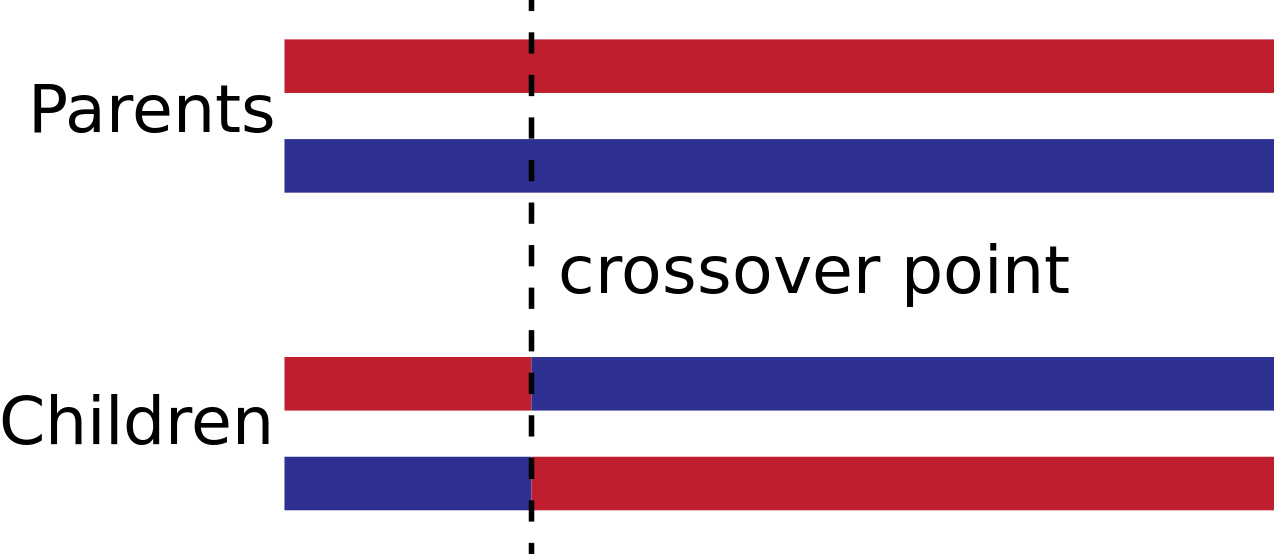
\includegraphics[scale=0.15]{Images/Chapter 9/crossover.png}
    \caption{Crossover in genetic algorithms}
    \source{R0oland on Wikipedia}
    \label{fig:ch9-crossover}
\end{figure}

\subsection{Mutation}
Mutation is a genetic operator used to maintain genetic diversity from one generation of a population of genetic algorithm chromosomes to the next. It alters one or more gene values in a chromosome from its initial state. The classic example of a mutation operator involves a probability that an arbitrary bit in a genetic sequence will be flipped from its original state.

The purpose of mutation in evolutionary algorithms is to introduce diversity into the sampled population. Mutation operators are used in an attempt to avoid local minima by preventing the population of chromosomes from becoming too similar to each other, thus slowing or even stopping convergence to the global optimum.

\subsection{Evaluation and replacement}
At each generation, the fitness of each individual is evaluated, and the population is usually replaced in its entirety by the offspring. Another possible solution is to keep the $n$ ``elite'' individuals from the previous generation to reduce the effects of mutations or sub-optimal fitness evaluation. 

\subsection{Coevolution}
Coevolution is an extension of evolutionary algorithms for domains with multiple agents. By using evolutionary algorithms, we can train a policy to perform a state-to-action mapping. In this approach, rather than update the parameters of a single agent interacting with the environment as it is done in reinforcement learning, one searches through a population of policies that have the highest fittest for the task at hand.
\chapter{Generative Machine Learning}
In the first chapter we said that in this course we would consider \textit{``machines that think, that learn and that create''}, following Herbert Simon’s definition of autonomous and adaptive systems. Until now we have focused on the first two points, discussing reinforcement learning and how we can build agents that take actions given a representation of the state. It is now time to move on to machines that \textit{create}.

Can machines even be creative? We will now see a few examples of generative models but let us always keep in mind the definition of \textbf{creativity} given by Margaret Ann Boden, a research professor of cognitive science at the University of Sussex: \textit{``Creativity can be defined as the ability to generate novel, and valuable, ideas. Valuable, here, has many meanings: interesting, useful, beautiful, simple, richly complex, and so on. Ideas covers many meanings too: not only ideas as such (concepts, theories, interpretations, stories), but also artifacts such as graphic images, sculptures, houses, and jet engines. Computer models have been designed to generate ideas in all these areas and more''}.

\section{Generative modeling}
\textbf{Generative models} are a class of statistical models that allow for the generation of new data instances. Given a set of data instances $X$ and a set of labels $Y$, they capture the joint probability $p(X,Y)$, or just $p(X)$ if there are no labels\footnote{From \url{https://developers.google.com/machine-learning/gan/generative}}. An example of such models are ones that predict the next word in a sequence. 

These models, however, tend to generate data that is just a variation of the one that has been used to train them, not meeting the novelty criterion we have presented earlier on. Given a dataset $\boldsymbol{X}$, produced according to an unknown distribution $p_{data}$, we want to create a generative model $p_{model}$ that can be used to generate samples that look like they were drawn from $p_{data}$ while also being different enough to be considered novel.

\subsection{Deep Dream}
Deep Dream is a computer vision program created by Alexander Mordvintsev, Christopher Olah and Mike Tika in 2015. It uses a deep convolutional neural network to find and enhance patterns in images creating a dream-like appearance in deliberately over-processed images\footnote{From \url{https://en.wikipedia.org/wiki/DeepDream}}.

While interpretability is still an open question in the deep learning field, image classifiers do not suffer from the same issue. Each layer, in fact, extracts higher and higher-level features of the images in order to make its classification decision. This can be exploited by means of a technique known as \textit{gradient ascent in input space}: we apply gradient \textit{descent} to the value of the input image of a convolutional neural network so as to maximize the response of a specific filter, starting from a blank input image. The resulting input image will be one that the chosen filter is maximally responsive to.

The same technique is used in Deep Dream: one or more layers are chosen, and an input is built so as to maximize the excitement from those layers. If we give the network an actual image as an input instead of noise, the network will then modify the image to maximize the response of the layers we chose, outputting the ``hallucinogenic'' results Deep Dream is known for.

\begin{figure}
    \centering
    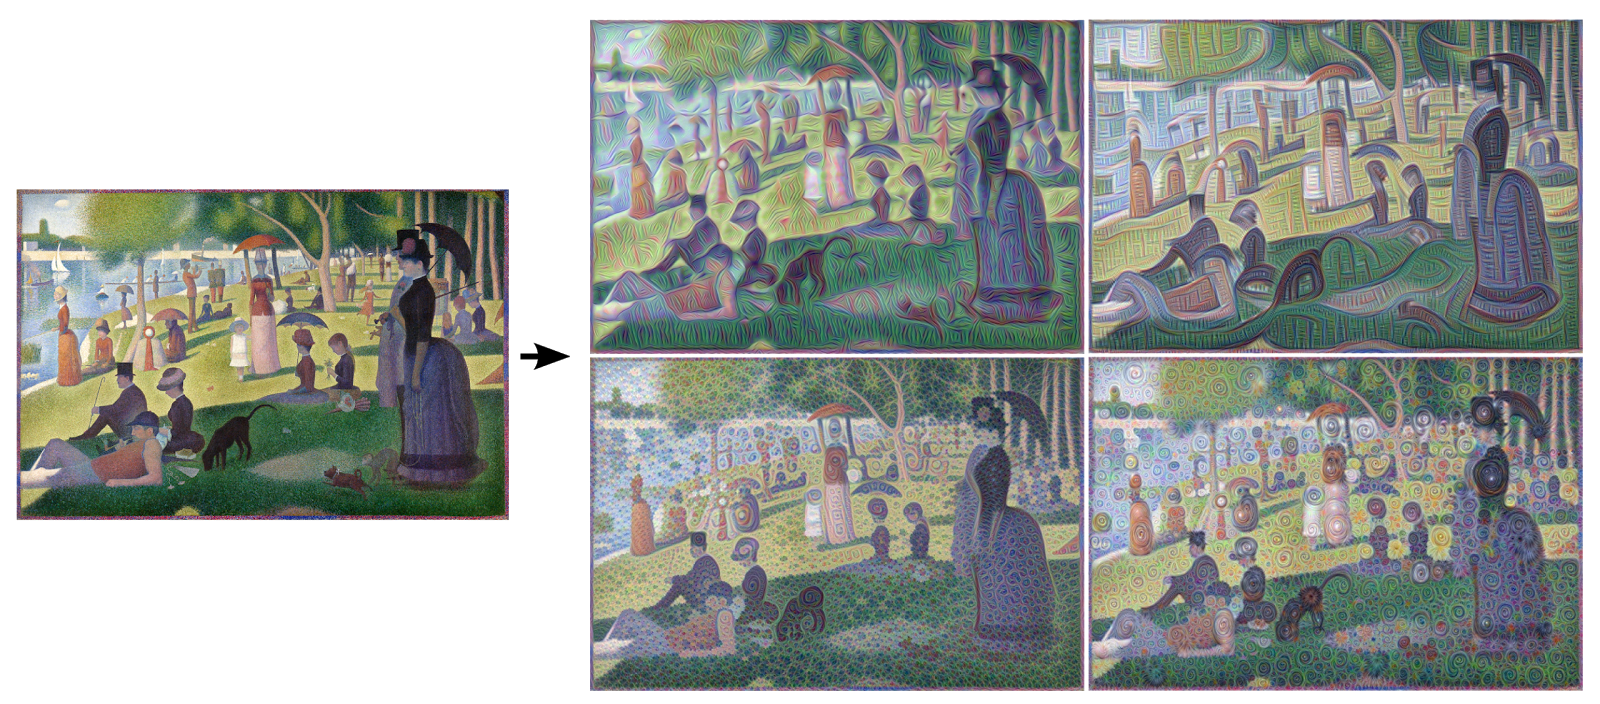
\includegraphics[scale=0.25]{Images/Chapter 10/deepdream.png}
    \caption{\textit{``A Sunday Afternoon on the Island of La Grande Jatte''} reimagined by DeepDream}
    \source{GoogleAI Blog}
    \label{fig:ch10-deepdream}
\end{figure}

\subsection{Generative Adversarial Networks}
Performing gradient ascent on a certain input image is not the only way for machines to create something original. Many of us will have probably come across the website ``This Person Does Not Exist''\footnote{\url{https://thispersondoesnotexist.com/}}, where we can see pictures of people that have been generated by a neural network called StyleGAN2.

GAN stands for Generative Adversarial Network, a class of machine learning frameworks designed by Ian Goodfellow and his colleagues in 2014 \cite{goodfellow2014generative}. They are made up of two neural networks: a \textbf{generative network}, responsible for generating candidates and a \textbf{discriminative network} that evaluates them. The objective of the generative network is to fool the discriminative network into believing that the image was part of the ground truth data used to train it\footnote{From: \url{https://en.wikipedia.org/wiki/Generative_adversarial_network}}.

\begin{figure}
    \centering
    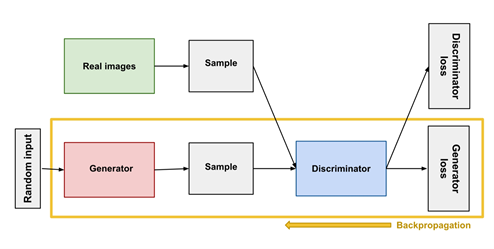
\includegraphics{Images/Chapter 10/gan.png}
    \caption{Structure of a Generative Adversarial Network}
    \source{Google Developers website}
    \label{fig:ch10-gan}
\end{figure}

\subsection{Text generation}
Neural networks can also generate text with great results. The latest and greatest example in these types of networks is GPT-3 (Generative Pre-trained Transformer 3), an autoregressive language model developed by OpenAI and published in May 2020. Trained with 175 billion parameters, it has been able to generate text with a quality so high that it difficult to distinguish from that written by a human.
\chapter{Autonomous robots and self-driving cars}
As we have seen in the first chapter, the term ``autonomous and adaptive systems'' is not limited to only software agents --like the ones that we have considered so far-- but it also encompasses physically situated \textbf{robots}.

After seeing some examples of unmanned robots (see slides 4-9 of the ``Autonomous Robots and Self-driving Cars'' slide deck), we ask two questions:

\begin{itemize}
    \item What is the difference between \textbf{automation} and \textbf{autonomy}?
    \item Why does it matter that there is a difference between autonomy and automation?
\end{itemize}

In first approximation we can say that \textit{automation} is about robots as tools, while \textit{autonomy} is about robots as agents. As it often happens, the line between the two is actually much more blurred. We present the following questions to help us discern between automation and autonomy:

\begin{itemize}
    \item Does the system focus on \textbf{executing} plans or on \textbf{generating} them?
    \item Does the system use a \textbf{closed} or an \textbf{open-world model}?
    \item Does the system use \textbf{deterministic} or \textbf{non-deterministic algorithms}?
    \item Does the system manipulate \textbf{signals} or \textbf{symbols/concepts}?
\end{itemize}

In many situations knowing the difference between the two terms is not enough, and we must choose which type of system to develop to best suit our needs. Automatic systems follow a deterministic behavior, making them predictable and, most importantly, testable. This may be sufficient for our use case, but in some instances we might want a certain degree of adaptability, through which the robot can autonomously handle unexpected changes without stopping. This degree of freedom must be kept in mind, and attention must be paid to the consequences of potential failures, both in terms of risks and liability for the damages that might be caused.

\section{World models}
Robots need to have a representation of the state around them, called a \textbf{world model}, to keep track of everything that is needed for their computation. The model may be pre-programmed and hard coded into the robot, or it may be learnt by the robot itself. It will not only include rules, constraints, and maps, but also beliefs and intentions.

If we work under the assumption that we know everything that might happen in our world, we are dealing with a \textbf{closed-world model} (e.g., any predicate that is not in our database is considered as false), in which we can specify in its entirety the list of possible states, objects and conditions. If this is not the case, we are working under an \textbf{open-world} hypothesis.

Closely related to these assumptions, we have the \textbf{frame problem}: how do we correctly identify the things that do not change over time in our world (e.g., walls, trees, etc.) to reduce computation? This is very important as it is linked to the concept of \textbf{bounded rationality}, originally introduced by Herbert Simon, stating that the decision-making capabilities of all agents (whether they are human or artificial) is limited by how much information they have, their computational abilities and the amount of time they have available to make a decision. We must also remember that, while a robot may dynamically adapt or change its plan of action to overcome the occurrence of unexpected events, it cannot go beyond what it has been programmed or trained for.

\section{Self-driving cars}
For the part on self-driving cars, refer to the slides.

% Bibliography
\clearpage
\printbibliography

\end{document}
